% Options for packages loaded elsewhere
\PassOptionsToPackage{unicode}{hyperref}
\PassOptionsToPackage{hyphens}{url}
%
\documentclass[
]{article}
\usepackage{amsmath,amssymb}
\usepackage{iftex}
\ifPDFTeX
  \usepackage[T1]{fontenc}
  \usepackage[utf8]{inputenc}
  \usepackage{textcomp} % provide euro and other symbols
\else % if luatex or xetex
  \usepackage{unicode-math} % this also loads fontspec
  \defaultfontfeatures{Scale=MatchLowercase}
  \defaultfontfeatures[\rmfamily]{Ligatures=TeX,Scale=1}
\fi
\usepackage{lmodern}
\ifPDFTeX\else
  % xetex/luatex font selection
\fi
% Use upquote if available, for straight quotes in verbatim environments
\IfFileExists{upquote.sty}{\usepackage{upquote}}{}
\IfFileExists{microtype.sty}{% use microtype if available
  \usepackage[]{microtype}
  \UseMicrotypeSet[protrusion]{basicmath} % disable protrusion for tt fonts
}{}
\makeatletter
\@ifundefined{KOMAClassName}{% if non-KOMA class
  \IfFileExists{parskip.sty}{%
    \usepackage{parskip}
  }{% else
    \setlength{\parindent}{0pt}
    \setlength{\parskip}{6pt plus 2pt minus 1pt}}
}{% if KOMA class
  \KOMAoptions{parskip=half}}
\makeatother
\usepackage{xcolor}
\usepackage[margin=1in]{geometry}
\usepackage{color}
\usepackage{fancyvrb}
\newcommand{\VerbBar}{|}
\newcommand{\VERB}{\Verb[commandchars=\\\{\}]}
\DefineVerbatimEnvironment{Highlighting}{Verbatim}{commandchars=\\\{\}}
% Add ',fontsize=\small' for more characters per line
\usepackage{framed}
\definecolor{shadecolor}{RGB}{248,248,248}
\newenvironment{Shaded}{\begin{snugshade}}{\end{snugshade}}
\newcommand{\AlertTok}[1]{\textcolor[rgb]{0.94,0.16,0.16}{#1}}
\newcommand{\AnnotationTok}[1]{\textcolor[rgb]{0.56,0.35,0.01}{\textbf{\textit{#1}}}}
\newcommand{\AttributeTok}[1]{\textcolor[rgb]{0.13,0.29,0.53}{#1}}
\newcommand{\BaseNTok}[1]{\textcolor[rgb]{0.00,0.00,0.81}{#1}}
\newcommand{\BuiltInTok}[1]{#1}
\newcommand{\CharTok}[1]{\textcolor[rgb]{0.31,0.60,0.02}{#1}}
\newcommand{\CommentTok}[1]{\textcolor[rgb]{0.56,0.35,0.01}{\textit{#1}}}
\newcommand{\CommentVarTok}[1]{\textcolor[rgb]{0.56,0.35,0.01}{\textbf{\textit{#1}}}}
\newcommand{\ConstantTok}[1]{\textcolor[rgb]{0.56,0.35,0.01}{#1}}
\newcommand{\ControlFlowTok}[1]{\textcolor[rgb]{0.13,0.29,0.53}{\textbf{#1}}}
\newcommand{\DataTypeTok}[1]{\textcolor[rgb]{0.13,0.29,0.53}{#1}}
\newcommand{\DecValTok}[1]{\textcolor[rgb]{0.00,0.00,0.81}{#1}}
\newcommand{\DocumentationTok}[1]{\textcolor[rgb]{0.56,0.35,0.01}{\textbf{\textit{#1}}}}
\newcommand{\ErrorTok}[1]{\textcolor[rgb]{0.64,0.00,0.00}{\textbf{#1}}}
\newcommand{\ExtensionTok}[1]{#1}
\newcommand{\FloatTok}[1]{\textcolor[rgb]{0.00,0.00,0.81}{#1}}
\newcommand{\FunctionTok}[1]{\textcolor[rgb]{0.13,0.29,0.53}{\textbf{#1}}}
\newcommand{\ImportTok}[1]{#1}
\newcommand{\InformationTok}[1]{\textcolor[rgb]{0.56,0.35,0.01}{\textbf{\textit{#1}}}}
\newcommand{\KeywordTok}[1]{\textcolor[rgb]{0.13,0.29,0.53}{\textbf{#1}}}
\newcommand{\NormalTok}[1]{#1}
\newcommand{\OperatorTok}[1]{\textcolor[rgb]{0.81,0.36,0.00}{\textbf{#1}}}
\newcommand{\OtherTok}[1]{\textcolor[rgb]{0.56,0.35,0.01}{#1}}
\newcommand{\PreprocessorTok}[1]{\textcolor[rgb]{0.56,0.35,0.01}{\textit{#1}}}
\newcommand{\RegionMarkerTok}[1]{#1}
\newcommand{\SpecialCharTok}[1]{\textcolor[rgb]{0.81,0.36,0.00}{\textbf{#1}}}
\newcommand{\SpecialStringTok}[1]{\textcolor[rgb]{0.31,0.60,0.02}{#1}}
\newcommand{\StringTok}[1]{\textcolor[rgb]{0.31,0.60,0.02}{#1}}
\newcommand{\VariableTok}[1]{\textcolor[rgb]{0.00,0.00,0.00}{#1}}
\newcommand{\VerbatimStringTok}[1]{\textcolor[rgb]{0.31,0.60,0.02}{#1}}
\newcommand{\WarningTok}[1]{\textcolor[rgb]{0.56,0.35,0.01}{\textbf{\textit{#1}}}}
\usepackage{longtable,booktabs,array}
\usepackage{calc} % for calculating minipage widths
% Correct order of tables after \paragraph or \subparagraph
\usepackage{etoolbox}
\makeatletter
\patchcmd\longtable{\par}{\if@noskipsec\mbox{}\fi\par}{}{}
\makeatother
% Allow footnotes in longtable head/foot
\IfFileExists{footnotehyper.sty}{\usepackage{footnotehyper}}{\usepackage{footnote}}
\makesavenoteenv{longtable}
\usepackage{graphicx}
\makeatletter
\def\maxwidth{\ifdim\Gin@nat@width>\linewidth\linewidth\else\Gin@nat@width\fi}
\def\maxheight{\ifdim\Gin@nat@height>\textheight\textheight\else\Gin@nat@height\fi}
\makeatother
% Scale images if necessary, so that they will not overflow the page
% margins by default, and it is still possible to overwrite the defaults
% using explicit options in \includegraphics[width, height, ...]{}
\setkeys{Gin}{width=\maxwidth,height=\maxheight,keepaspectratio}
% Set default figure placement to htbp
\makeatletter
\def\fps@figure{htbp}
\makeatother
\setlength{\emergencystretch}{3em} % prevent overfull lines
\providecommand{\tightlist}{%
  \setlength{\itemsep}{0pt}\setlength{\parskip}{0pt}}
\setcounter{secnumdepth}{-\maxdimen} % remove section numbering
\usepackage{booktabs}
\usepackage{longtable}
\usepackage{array}
\usepackage{multirow}
\usepackage{wrapfig}
\usepackage{float}
\usepackage{colortbl}
\usepackage{pdflscape}
\usepackage{tabu}
\usepackage{threeparttable}
\usepackage{threeparttablex}
\usepackage[normalem]{ulem}
\usepackage{makecell}
\usepackage{xcolor}
\usepackage{multicol}
\usepackage{hhline}
\newlength\Oldarrayrulewidth
\newlength\Oldtabcolsep
\usepackage{hyperref}
\ifLuaTeX
  \usepackage{selnolig}  % disable illegal ligatures
\fi
\IfFileExists{bookmark.sty}{\usepackage{bookmark}}{\usepackage{hyperref}}
\IfFileExists{xurl.sty}{\usepackage{xurl}}{} % add URL line breaks if available
\urlstyle{same}
\hypersetup{
  hidelinks,
  pdfcreator={LaTeX via pandoc}}

\author{}
\date{\vspace{-2.5em}}

\begin{document}

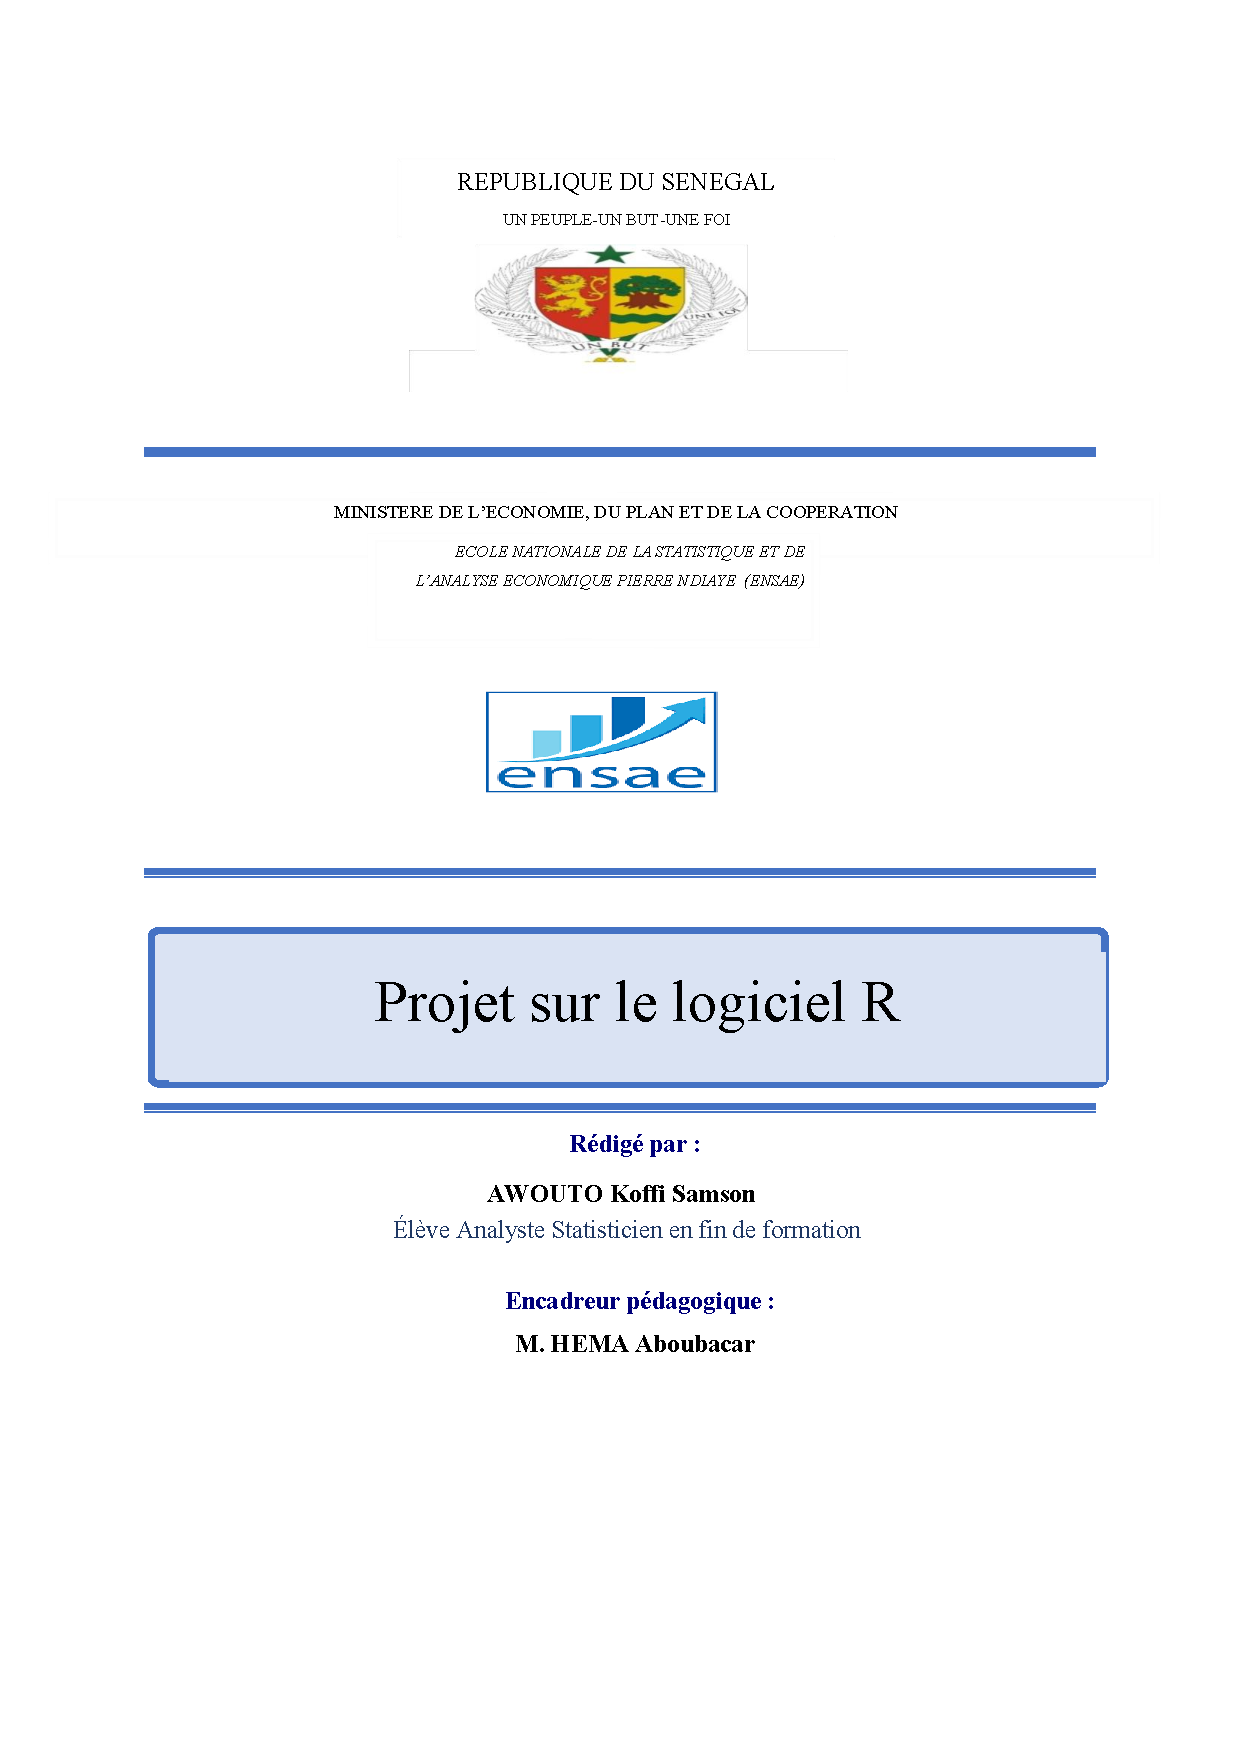
\includepdf{PAGE DE GARDE TP_R.pdf}
\setcounter{tocdepth}{4}        
\renewcommand{\contentsname}{\textcolor{blue}{Table des Matières}}

\textcolor{black}{\tableofcontents} \newpage

\begin{Shaded}
\begin{Highlighting}[]
\NormalTok{knitr}\SpecialCharTok{::}\NormalTok{opts\_chunk}\SpecialCharTok{$}\FunctionTok{set}\NormalTok{(}\AttributeTok{echo =} \ConstantTok{TRUE}\NormalTok{, }\AttributeTok{warning =} \ConstantTok{FALSE}\NormalTok{, }\AttributeTok{error =} \ConstantTok{FALSE}\NormalTok{,}\AttributeTok{message =} \ConstantTok{FALSE}\NormalTok{)}
\end{Highlighting}
\end{Shaded}

\begin{Shaded}
\begin{Highlighting}[]
\CommentTok{\# les packages à installer }

\CommentTok{\#install.packages("gtsummary")}
\CommentTok{\#install.packages("janitor")}
\CommentTok{\#install.packages("ggplot2")}
\CommentTok{\#install.packages("webshot")}
\CommentTok{\#install.packages("readxl")}
\CommentTok{\#install.packages("gridExtra")}
\CommentTok{\#install.packages("ggExtra")}
\CommentTok{\#install.packages("flextable")}
\end{Highlighting}
\end{Shaded}

\begin{Shaded}
\begin{Highlighting}[]
\FunctionTok{library}\NormalTok{(gtsummary)}
\FunctionTok{library}\NormalTok{(janitor)}
\FunctionTok{library}\NormalTok{(dplyr)}
\FunctionTok{library}\NormalTok{(gt)}
\FunctionTok{library}\NormalTok{(ggplot2)}
\FunctionTok{library}\NormalTok{(flextable)}
\CommentTok{\#library(htmlwidgets)}
\FunctionTok{library}\NormalTok{(webshot)}
\FunctionTok{library}\NormalTok{(readxl)}
\FunctionTok{library}\NormalTok{(knitr)}
\FunctionTok{library}\NormalTok{(lubridate)}
\FunctionTok{library}\NormalTok{(gridExtra)}
\FunctionTok{library}\NormalTok{(ggExtra)}
\end{Highlighting}
\end{Shaded}

\hypertarget{partie-1}{%
\section{1. Partie 1}\label{partie-1}}

\hypertarget{pruxe9paration-des-donnuxe9es}{%
\subsection{1.1. Préparation des
données}\label{pruxe9paration-des-donnuxe9es}}

\hypertarget{importation-et-mise-en-forme}{%
\subsubsection{1.1.1. Importation et mise en
forme}\label{importation-et-mise-en-forme}}

\hypertarget{importation-de-la-base}{%
\paragraph{1.1.1.1. Importation de la
base}\label{importation-de-la-base}}

\begin{Shaded}
\begin{Highlighting}[]
\FunctionTok{library}\NormalTok{(readxl)}
\FunctionTok{getwd}\NormalTok{()}
\end{Highlighting}
\end{Shaded}

\begin{verbatim}
## [1] "C:/Users/SAMSON/Documents/AWOUTO_SAMSON_PROJET_R"
\end{verbatim}

\begin{Shaded}
\begin{Highlighting}[]
\NormalTok{projet }\OtherTok{\textless{}{-}} \FunctionTok{read\_excel}\NormalTok{(}\StringTok{"Base\_Projet.xlsx"}\NormalTok{)}
\end{Highlighting}
\end{Shaded}

\hypertarget{nombre-de-lignes-et-de-colonnes-de-la-base-projet}{%
\paragraph{1.1.1.2. Nombre de lignes et de colonnes de la base
projet}\label{nombre-de-lignes-et-de-colonnes-de-la-base-projet}}

\begin{Shaded}
\begin{Highlighting}[]
\NormalTok{nb\_lignes }\OtherTok{\textless{}{-}} \FunctionTok{nrow}\NormalTok{(projet)}
\NormalTok{nb\_colonnes }\OtherTok{\textless{}{-}} \FunctionTok{ncol}\NormalTok{(projet)}
\FunctionTok{cat}\NormalTok{(}\StringTok{"Nombre de lignes (PME) :"}\NormalTok{, nb\_lignes, }\StringTok{"}\SpecialCharTok{\textbackslash{}n}\StringTok{"}\NormalTok{)}
\end{Highlighting}
\end{Shaded}

\begin{verbatim}
## Nombre de lignes (PME) : 250
\end{verbatim}

\begin{Shaded}
\begin{Highlighting}[]
\FunctionTok{cat}\NormalTok{(}\StringTok{"Nombre de colonnes (variables) :"}\NormalTok{, nb\_colonnes, }\StringTok{"}\SpecialCharTok{\textbackslash{}n}\StringTok{"}\NormalTok{)}
\end{Highlighting}
\end{Shaded}

\begin{verbatim}
## Nombre de colonnes (variables) : 33
\end{verbatim}

\hypertarget{vuxe9rification-des-valeurs-manquantes-pour-la-variable-key-dans-la-base-projet}{%
\paragraph{1.1.1.3. Vérification des valeurs manquantes pour la variable
key dans la base
projet}\label{vuxe9rification-des-valeurs-manquantes-pour-la-variable-key-dans-la-base-projet}}

\begin{Shaded}
\begin{Highlighting}[]
\ControlFlowTok{if}\NormalTok{ (}\FunctionTok{any}\NormalTok{(}\FunctionTok{is.na}\NormalTok{(projet}\SpecialCharTok{$}\NormalTok{key))) \{}
  \FunctionTok{cat}\NormalTok{(}\StringTok{"Il y a des valeurs manquantes pour la variable \textquotesingle{}key\textquotesingle{}.}\SpecialCharTok{\textbackslash{}n}\StringTok{"}\NormalTok{)}
  \CommentTok{\# Identifier les lignes avec des valeurs manquantes pour \textquotesingle{}key\textquotesingle{}}
\NormalTok{  pme\_manquantes }\OtherTok{\textless{}{-}}\NormalTok{ projet}\SpecialCharTok{$}\NormalTok{key[}\FunctionTok{is.na}\NormalTok{(projet}\SpecialCharTok{$}\NormalTok{key)]}
  \FunctionTok{cat}\NormalTok{(}\StringTok{"Les PME concernées sont :"}\NormalTok{, }\FunctionTok{paste}\NormalTok{(pme\_manquantes, }\AttributeTok{collapse =} \StringTok{", "}\NormalTok{), }\StringTok{"}\SpecialCharTok{\textbackslash{}n}\StringTok{"}\NormalTok{)}
\NormalTok{\} }\ControlFlowTok{else}\NormalTok{ \{}
  \FunctionTok{cat}\NormalTok{(}\StringTok{"Il n\textquotesingle{}y a pas de valeurs manquantes pour la variable \textquotesingle{}key\textquotesingle{}.}\SpecialCharTok{\textbackslash{}n}\StringTok{"}\NormalTok{)}
  
\NormalTok{\}}
\end{Highlighting}
\end{Shaded}

\begin{verbatim}
## Il n'y a pas de valeurs manquantes pour la variable 'key'.
\end{verbatim}

\begin{verbatim}
 De ce qui précède, on est certain que chaque les individus 
 de la base de  données possède  un identifiant
\end{verbatim}

\hypertarget{cruxe9ation-de-variables}{%
\subsubsection{1.1.2. Création de
variables}\label{cruxe9ation-de-variables}}

\hypertarget{renommage}{%
\paragraph{1.1.2.1. Renommage}\label{renommage}}

\begin{Shaded}
\begin{Highlighting}[]
\FunctionTok{library}\NormalTok{(dplyr)}


\NormalTok{projet }\OtherTok{\textless{}{-}}\NormalTok{ projet }\SpecialCharTok{\%\textgreater{}\%}
\NormalTok{  dplyr}\SpecialCharTok{::}\FunctionTok{rename}\NormalTok{(}\AttributeTok{region =}\NormalTok{ q1,}
         \AttributeTok{departement =}\NormalTok{ q2,}
         \AttributeTok{sexe =}\NormalTok{ q23)}
\end{Highlighting}
\end{Shaded}

\begin{Shaded}
\begin{Highlighting}[]
\CommentTok{\# Création d\textquotesingle{}une base de donnée alternative pour préserver la bse initiale}
\NormalTok{Projet }\OtherTok{\textless{}{-}}\NormalTok{ projet}
\end{Highlighting}
\end{Shaded}

\hypertarget{cruxe9ation-de-la-variable-sexe_2}{%
\paragraph{1.1.2.2. Création de la variable
sexe\_2}\label{cruxe9ation-de-la-variable-sexe_2}}

\begin{Shaded}
\begin{Highlighting}[]
\NormalTok{projet }\OtherTok{\textless{}{-}}\NormalTok{ projet }\SpecialCharTok{\%\textgreater{}\%}
  \FunctionTok{mutate}\NormalTok{(}\AttributeTok{sexe\_2 =} \FunctionTok{factor}\NormalTok{(}\FunctionTok{case\_when}\NormalTok{(sexe }\SpecialCharTok{==} \StringTok{"Femme"} \SpecialCharTok{\textasciitilde{}} \DecValTok{1}\NormalTok{, }\ConstantTok{TRUE} \SpecialCharTok{\textasciitilde{}} \DecValTok{0}\NormalTok{)))}

\CommentTok{\# Créer un data.frame nommé langues}
\NormalTok{langues }\OtherTok{\textless{}{-}} \FunctionTok{data.frame}\NormalTok{(projet }\SpecialCharTok{\%\textgreater{}\%}
  \FunctionTok{select}\NormalTok{(key, }\FunctionTok{starts\_with}\NormalTok{(}\StringTok{"q24a\_"}\NormalTok{)))}
\end{Highlighting}
\end{Shaded}

\hypertarget{cruxe9eation-dune-variable-nommuxe9e-parle}{%
\paragraph{1.1.2.3.Créeation d'une variable nommée
``parle''}\label{cruxe9eation-dune-variable-nommuxe9e-parle}}

\begin{Shaded}
\begin{Highlighting}[]
\NormalTok{langue }\OtherTok{\textless{}{-}}\NormalTok{ langues }\SpecialCharTok{\%\textgreater{}\%}
  \FunctionTok{mutate}\NormalTok{(}\AttributeTok{parle =} \FunctionTok{rowSums}\NormalTok{(}\FunctionTok{select}\NormalTok{(langues, }\FunctionTok{starts\_with}\NormalTok{(}\StringTok{"q24a\_"}\NormalTok{))))}
\end{Highlighting}
\end{Shaded}

\hypertarget{suxe9lectionn-exclusive-des-variables-key-et-parle}{%
\paragraph{1.1.2.3.Sélectionn exclusive des variables ``key'' et
``parle''}\label{suxe9lectionn-exclusive-des-variables-key-et-parle}}

\begin{Shaded}
\begin{Highlighting}[]
\NormalTok{langues }\OtherTok{\textless{}{-}}\NormalTok{ langue }\SpecialCharTok{\%\textgreater{}\%}
  \FunctionTok{select}\NormalTok{(key, parle)}

\CommentTok{\# Fusionner les data.frames projet et langues}
\NormalTok{projet }\OtherTok{\textless{}{-}} \FunctionTok{left\_join}\NormalTok{(projet, langues, }\AttributeTok{by =} \StringTok{"key"}\NormalTok{)}
\end{Highlighting}
\end{Shaded}

\hypertarget{statistiques-descriptives}{%
\section{2. Statistiques Descriptives}\label{statistiques-descriptives}}

\hypertarget{cruxe9ation-des-fonction}{%
\subsection{2.1. Création des fonction}\label{cruxe9ation-des-fonction}}

\hypertarget{premiuxe8re-fonction-univariuxe9e}{%
\paragraph{2.1.1. première fonction
univariée}\label{premiuxe8re-fonction-univariuxe9e}}

Cette fonction permet de générer des tableuax d'une variables donnée
dans une base de données

\begin{Shaded}
\begin{Highlighting}[]
\FunctionTok{library}\NormalTok{(knitr)}
\FunctionTok{library}\NormalTok{(kableExtra)}

\NormalTok{univarie\_1 }\OtherTok{\textless{}{-}} \ControlFlowTok{function}\NormalTok{(variable, }\AttributeTok{base\_de\_donnees =} \StringTok{""}\NormalTok{) \{}
  \CommentTok{\# Calculer la fréquence absolue}
\NormalTok{  freq\_absolue }\OtherTok{\textless{}{-}} \FunctionTok{table}\NormalTok{(variable)}
  
  \CommentTok{\# Calculer la fréquence relative avec deux chiffres après la virgule}
\NormalTok{  freq\_relative }\OtherTok{\textless{}{-}} \FunctionTok{round}\NormalTok{(}\FunctionTok{prop.table}\NormalTok{(freq\_absolue), }\DecValTok{2}\NormalTok{)}
  
  \CommentTok{\# Créer le tableau de distribution}
\NormalTok{  tableau }\OtherTok{\textless{}{-}} \FunctionTok{data.frame}\NormalTok{(Modalités }\OtherTok{=} \FunctionTok{as.character}\NormalTok{(}\FunctionTok{names}\NormalTok{(freq\_absolue)),}
                        \AttributeTok{Effectif =} \FunctionTok{as.vector}\NormalTok{(freq\_absolue),}
\NormalTok{                        Fréquence }\OtherTok{=} \FunctionTok{as.vector}\NormalTok{(freq\_relative))}
  
  \CommentTok{\# Calculer le total des fréquences absolues}
\NormalTok{  total\_freq\_absolue }\OtherTok{\textless{}{-}} \FunctionTok{sum}\NormalTok{(freq\_absolue)}
  
  \CommentTok{\# Ajouter la ligne du total}
\NormalTok{  total\_row }\OtherTok{\textless{}{-}} \FunctionTok{c}\NormalTok{(}\StringTok{"Total"}\NormalTok{, total\_freq\_absolue, }\DecValTok{1}\NormalTok{)}
\NormalTok{  tableau }\OtherTok{\textless{}{-}} \FunctionTok{rbind}\NormalTok{(tableau, total\_row)}
  
  \CommentTok{\# Afficher le tableau de distribution avec kableExtra}
\NormalTok{  knitr}\SpecialCharTok{::}\FunctionTok{kable}\NormalTok{(tableau, }\AttributeTok{align =} \StringTok{"c"}\NormalTok{, }\AttributeTok{caption =} \StringTok{"Tableau de distribution des fréquences"}\NormalTok{) }\SpecialCharTok{\%\textgreater{}\%}
    \FunctionTok{kable\_styling}\NormalTok{(}\AttributeTok{bootstrap\_options =} \StringTok{"striped"}\NormalTok{, }\AttributeTok{full\_width =} \ConstantTok{FALSE}\NormalTok{) }\SpecialCharTok{\%\textgreater{}\%}
    \FunctionTok{add\_header\_above}\NormalTok{(}\FunctionTok{c}\NormalTok{(}\StringTok{" "}\NormalTok{, }\StringTok{"Fréquences"} \OtherTok{=} \DecValTok{2}\NormalTok{)) }\SpecialCharTok{\%\textgreater{}\%}
    \FunctionTok{row\_spec}\NormalTok{(}\FunctionTok{nrow}\NormalTok{(tableau), }\AttributeTok{bold =} \ConstantTok{TRUE}\NormalTok{)}
\NormalTok{\}}
\end{Highlighting}
\end{Shaded}

\hypertarget{deuxiuxe8me-fonction-univariuxe9e}{%
\paragraph{2.1.1.deuxième fonction
univariée}\label{deuxiuxe8me-fonction-univariuxe9e}}

Cette fonction permet de générer un graphque en barre ou un diagramme
circulaire en fonction de l'option qu'aurait chosis l'utilisateu. On a
en effet l'option barreet l'option \emph{cercle}(diagramme circulaire)
et \emph{barre}(diagramme en barre)

\begin{Shaded}
\begin{Highlighting}[]
\FunctionTok{library}\NormalTok{(ggplot2)}

\NormalTok{univarié\_graphique}\OtherTok{\textless{}{-}} \ControlFlowTok{function}\NormalTok{(variable, }\AttributeTok{type\_graphique =} \StringTok{"barres"}\NormalTok{) \{}
  \CommentTok{\# Calculer la fréquence absolue}
\NormalTok{  freq\_absolue }\OtherTok{\textless{}{-}} \FunctionTok{table}\NormalTok{(variable)}
  
  \CommentTok{\# Calculer la fréquence relative en pourcentage avec deux chiffres après la virgule}
\NormalTok{  freq\_relative }\OtherTok{\textless{}{-}} \FunctionTok{prop.table}\NormalTok{(freq\_absolue) }\SpecialCharTok{*} \DecValTok{100}
  
  \CommentTok{\# Créer un dataframe à partir des fréquences absolues et relatives}
\NormalTok{  df }\OtherTok{\textless{}{-}} \FunctionTok{data.frame}\NormalTok{(Modalité }\OtherTok{=} \FunctionTok{as.character}\NormalTok{(}\FunctionTok{names}\NormalTok{(freq\_absolue)),}
\NormalTok{                   Fréquence}\AttributeTok{\_Absolue =} \FunctionTok{as.vector}\NormalTok{(freq\_absolue),}
\NormalTok{                   Fréquence}\AttributeTok{\_Relative =} \FunctionTok{as.vector}\NormalTok{(freq\_relative))}
  
  \CommentTok{\# Formatage des fréquences relatives avec deux chiffres après la virgule}
\NormalTok{  df}\SpecialCharTok{$}\NormalTok{Fréquence\_Relative }\OtherTok{\textless{}{-}} \FunctionTok{paste0}\NormalTok{(}\FunctionTok{format}\NormalTok{(}\FunctionTok{round}\NormalTok{(df}\SpecialCharTok{$}\NormalTok{Fréquence\_Relative, }\DecValTok{2}\NormalTok{), }\AttributeTok{nsmall =} \DecValTok{2}\NormalTok{), }\StringTok{"\%"}\NormalTok{)}
  
  \CommentTok{\# Créer le graphique en barres avec des couleurs variées}
  \ControlFlowTok{if}\NormalTok{ (type\_graphique }\SpecialCharTok{==} \StringTok{"barres"}\NormalTok{) \{}
    \FunctionTok{ggplot}\NormalTok{(df, }\FunctionTok{aes}\NormalTok{(}\AttributeTok{x =}\NormalTok{ Modalité, }\AttributeTok{y =}\NormalTok{ Fréquence\_Absolue, }\AttributeTok{fill =}\NormalTok{ Modalité)) }\SpecialCharTok{+}
      \FunctionTok{geom\_bar}\NormalTok{(}\AttributeTok{stat =} \StringTok{"identity"}\NormalTok{) }\SpecialCharTok{+}
      \FunctionTok{geom\_text}\NormalTok{(}\FunctionTok{aes}\NormalTok{(}\AttributeTok{label =}\NormalTok{ Fréquence\_Relative), }\AttributeTok{vjust =} \SpecialCharTok{{-}}\FloatTok{0.5}\NormalTok{, }\AttributeTok{size =} \DecValTok{3}\NormalTok{) }\SpecialCharTok{+} \CommentTok{\# Ajout des fréquences relatives}
      \FunctionTok{labs}\NormalTok{(}\AttributeTok{title =} \StringTok{"Graphique en Barres"}\NormalTok{, }\AttributeTok{x =} \StringTok{"Modalité"}\NormalTok{, }\AttributeTok{y =} \StringTok{"Fréquence Absolue"}\NormalTok{) }\SpecialCharTok{+}
      \FunctionTok{theme\_minimal}\NormalTok{() }\SpecialCharTok{+}
      \FunctionTok{scale\_fill\_hue}\NormalTok{(}\AttributeTok{name =} \StringTok{"Modalité"}\NormalTok{)}
\NormalTok{  \} }\ControlFlowTok{else} \ControlFlowTok{if}\NormalTok{ (type\_graphique }\SpecialCharTok{==} \StringTok{"cercle"}\NormalTok{) \{}
    \CommentTok{\# Créer le graphique circulaire avec des couleurs variées}
    \FunctionTok{ggplot}\NormalTok{(df, }\FunctionTok{aes}\NormalTok{(}\AttributeTok{x =} \StringTok{""}\NormalTok{, }\AttributeTok{y =}\NormalTok{ Fréquence\_Relative, }\AttributeTok{fill =}\NormalTok{ Modalité)) }\SpecialCharTok{+}
      \FunctionTok{geom\_bar}\NormalTok{(}\AttributeTok{stat =} \StringTok{"identity"}\NormalTok{, }\AttributeTok{width =} \DecValTok{1}\NormalTok{) }\SpecialCharTok{+}
      \FunctionTok{geom\_text}\NormalTok{(}\FunctionTok{aes}\NormalTok{(}\AttributeTok{label =}\NormalTok{ Fréquence\_Relative), }\AttributeTok{position =} \FunctionTok{position\_stack}\NormalTok{(}\AttributeTok{vjust =} \FloatTok{0.5}\NormalTok{), }\AttributeTok{size =} \DecValTok{3}\NormalTok{) }\SpecialCharTok{+} \CommentTok{\# Ajout des fréquences relatives}
      \FunctionTok{coord\_polar}\NormalTok{(}\StringTok{"y"}\NormalTok{, }\AttributeTok{start =} \DecValTok{0}\NormalTok{) }\SpecialCharTok{+}
      \FunctionTok{labs}\NormalTok{(}\AttributeTok{title =} \StringTok{"Graphique Circulaire"}\NormalTok{, }\AttributeTok{fill =} \StringTok{"Modalité"}\NormalTok{) }\SpecialCharTok{+}
      \FunctionTok{theme\_minimal}\NormalTok{() }\SpecialCharTok{+}
      \FunctionTok{theme}\NormalTok{(}\AttributeTok{axis.title.x=}\FunctionTok{element\_blank}\NormalTok{(),}
            \AttributeTok{axis.text.x=}\FunctionTok{element\_blank}\NormalTok{(),}
            \AttributeTok{axis.ticks.x=}\FunctionTok{element\_blank}\NormalTok{()) }\SpecialCharTok{+}
      \FunctionTok{scale\_fill\_hue}\NormalTok{(}\AttributeTok{name =} \StringTok{"Modalité"}\NormalTok{)}
\NormalTok{  \} }\ControlFlowTok{else}\NormalTok{ \{}
    \FunctionTok{cat}\NormalTok{(}\StringTok{"Type de graphique non reconnu. Veuillez spécifier \textquotesingle{}barres\textquotesingle{} ou \textquotesingle{}cercle\textquotesingle{}."}\NormalTok{)}
\NormalTok{  \}}
\NormalTok{\}}

\CommentTok{\# Exemple d\textquotesingle{}utilisation}
\NormalTok{donnees }\OtherTok{\textless{}{-}} \FunctionTok{c}\NormalTok{(}\StringTok{"A"}\NormalTok{, }\StringTok{"A"}\NormalTok{, }\StringTok{"B"}\NormalTok{, }\StringTok{"C"}\NormalTok{, }\StringTok{"C"}\NormalTok{, }\StringTok{"C"}\NormalTok{, }\StringTok{"D"}\NormalTok{)}
\NormalTok{univarié}\FunctionTok{\_graphique}\NormalTok{(donnees, }\AttributeTok{type\_graphique =} \StringTok{"cercle"}\NormalTok{)}
\end{Highlighting}
\end{Shaded}

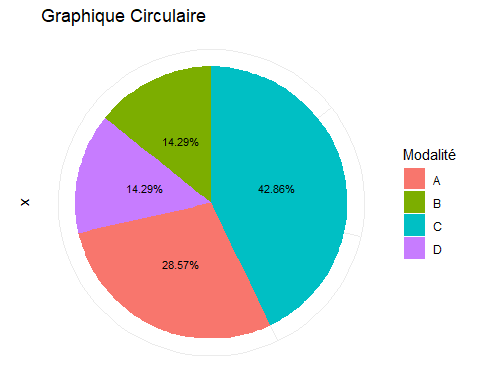
\includegraphics{AWOUTO_Projet_files/figure-latex/unnamed-chunk-12-1.pdf}

\hypertarget{cruxe9ation-de-la-fonction-bivariuxe9e}{%
\paragraph{2.1.3. Création de la fonction
bivariée}\label{cruxe9ation-de-la-fonction-bivariuxe9e}}

la fonction bivariée est nommée tableau\_croise et prend en argument
deux variables ,puis retourne un \emph{tableau croisé}

\begin{Shaded}
\begin{Highlighting}[]
\DocumentationTok{\#\#\# fonction bivariée: Fonction pour calculer les statistiques usuelles d\textquotesingle{}une variable quantitative}
\NormalTok{tableau\_croise }\OtherTok{\textless{}{-}} \ControlFlowTok{function}\NormalTok{(var1, var2) \{}
  \CommentTok{\# Calcul du tableau croisé}
\NormalTok{  tab }\OtherTok{\textless{}{-}} \FunctionTok{table}\NormalTok{(var1, var2)}
  
  \CommentTok{\# Ajout des totaux par ligne et par colonne}
\NormalTok{  tab\_with\_totals }\OtherTok{\textless{}{-}} \FunctionTok{addmargins}\NormalTok{(tab, }\DecValTok{1}\NormalTok{, }\AttributeTok{FUN =} \FunctionTok{list}\NormalTok{(}\AttributeTok{Total =}\NormalTok{ sum))}
\NormalTok{  tab\_with\_totals }\OtherTok{\textless{}{-}} \FunctionTok{addmargins}\NormalTok{(tab\_with\_totals, }\DecValTok{2}\NormalTok{, }\AttributeTok{FUN =} \FunctionTok{list}\NormalTok{(}\AttributeTok{Total =}\NormalTok{ sum))}
  
  \CommentTok{\# Renommer les dimensions pour une meilleure lisibilité}
  \FunctionTok{dimnames}\NormalTok{(tab\_with\_totals)[[}\DecValTok{1}\NormalTok{]][}\FunctionTok{dim}\NormalTok{(tab\_with\_totals)[}\DecValTok{1}\NormalTok{]] }\OtherTok{\textless{}{-}} \StringTok{"Total"}
  \FunctionTok{dimnames}\NormalTok{(tab\_with\_totals)[[}\DecValTok{2}\NormalTok{]][}\FunctionTok{dim}\NormalTok{(tab\_with\_totals)[}\DecValTok{2}\NormalTok{]] }\OtherTok{\textless{}{-}} \StringTok{"Total"}
  
  \FunctionTok{return}\NormalTok{(tab\_with\_totals)}
  
  

\NormalTok{\}}
\end{Highlighting}
\end{Shaded}

\hypertarget{la-repartition-des-proportion-suivants-les-variables-donnes}{%
\paragraph{2.1.4. LA REPARTITION DES PROPORTION SUIVANTS LES VARIABLES
DONNES}\label{la-repartition-des-proportion-suivants-les-variables-donnes}}

\hypertarget{recodage-de-certaines-variables-dintuxe9ruxeat}{%
\subparagraph{2.1.4.0 Recodage de certaines variables
d'intérêt}\label{recodage-de-certaines-variables-dintuxe9ruxeat}}

\begin{verbatim}
Dans cette partie nous avons trouvé judicuex de renommer les variables avec des     noms familiers pour uen lecture facile des statsitiques qui seront générées.
\end{verbatim}

\begin{Shaded}
\begin{Highlighting}[]
\CommentTok{\#recodons les variables importantes:}
\CommentTok{\# Renommer les variables q1, q2 et q23}
\NormalTok{projet }\OtherTok{\textless{}{-}}\NormalTok{ projet }\SpecialCharTok{\%\textgreater{}\%}
\NormalTok{  dplyr}\SpecialCharTok{::}\FunctionTok{rename}\NormalTok{(    }\StringTok{"Niveau d’instruction"} \OtherTok{=}\NormalTok{ q25,}
                   \StringTok{"Statut juridique"} \OtherTok{=}\NormalTok{q12,}
                  \StringTok{"propriétaire ou locataire"} \OtherTok{=}\NormalTok{ q81)}
\end{Highlighting}
\end{Shaded}

\hypertarget{repartition-des-pme-selon-le-sexe}{%
\subparagraph{2.1.4.1 Repartition des PME selon le
sexe}\label{repartition-des-pme-selon-le-sexe}}

\begin{Shaded}
\begin{Highlighting}[]
\CommentTok{\# repartition du sexe }
\FunctionTok{univarie\_1}\NormalTok{(projet}\SpecialCharTok{$}\NormalTok{sexe, projet)}
\end{Highlighting}
\end{Shaded}

\begin{longtable}[t]{ccc}
\caption{\label{tab:unnamed-chunk-15}Tableau de distribution des fréquences}\\
\toprule
\multicolumn{1}{c}{ } & \multicolumn{2}{c}{Fréquences} \\
\cmidrule(l{3pt}r{3pt}){2-3}
Modalités & Effectif & Fréquence\\
\midrule
Femme & 191 & 0.76\\
Homme & 59 & 0.24\\
\textbf{Total} & \textbf{250} & \textbf{1}\\
\bottomrule
\end{longtable}

\begin{Shaded}
\begin{Highlighting}[]
\NormalTok{univarié}\FunctionTok{\_graphique}\NormalTok{(projet}\SpecialCharTok{$}\NormalTok{sexe , }\StringTok{"barres"}\NormalTok{)}
\end{Highlighting}
\end{Shaded}

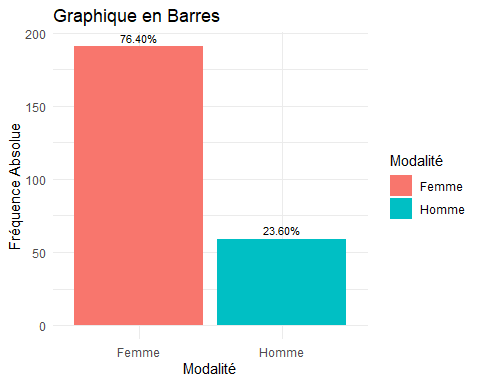
\includegraphics{AWOUTO_Projet_files/figure-latex/unnamed-chunk-15-1.pdf}

Du graphique ci-dessus , on note que les femmes sont les personnes les
plus nombresues dans l'échantillon prise pour les études soit 76\% des
PME contre 24\% pour les hommes

\hypertarget{repartition-des-pme-selon-le-niveau-dinstruction}{%
\subparagraph{2.1.4.2 Repartition des PME selon le Niveau
d'instruction}\label{repartition-des-pme-selon-le-niveau-dinstruction}}

\begin{Shaded}
\begin{Highlighting}[]
\FunctionTok{univarie\_1}\NormalTok{(projet}\SpecialCharTok{$}\StringTok{\textasciigrave{}}\AttributeTok{Niveau d’instruction}\StringTok{\textasciigrave{}}\NormalTok{, projet)}
\end{Highlighting}
\end{Shaded}

\begin{longtable}[t]{ccc}
\caption{\label{tab:unnamed-chunk-16}Tableau de distribution des fréquences}\\
\toprule
\multicolumn{1}{c}{ } & \multicolumn{2}{c}{Fréquences} \\
\cmidrule(l{3pt}r{3pt}){2-3}
Modalités & Effectif & Fréquence\\
\midrule
Aucun niveau & 79 & 0.32\\
Niveau primaire & 56 & 0.22\\
Niveau secondaire & 74 & 0.3\\
Niveau Superieur & 41 & 0.16\\
\textbf{Total} & \textbf{250} & \textbf{1}\\
\bottomrule
\end{longtable}

\begin{Shaded}
\begin{Highlighting}[]
\NormalTok{univarié}\FunctionTok{\_graphique}\NormalTok{(projet}\SpecialCharTok{$}\StringTok{\textasciigrave{}}\AttributeTok{Niveau d’instruction}\StringTok{\textasciigrave{}}\NormalTok{ , }\StringTok{"cercle"}\NormalTok{)}
\end{Highlighting}
\end{Shaded}

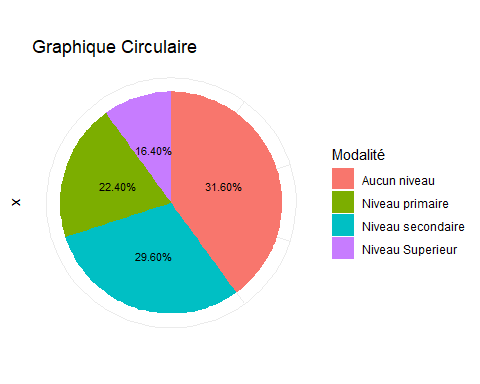
\includegraphics{AWOUTO_Projet_files/figure-latex/unnamed-chunk-16-1.pdf}

De ce graphique on retient essentiellement que les propriétaires des
plantations ou des champs n'ont pas en général pas pu effectuer des
études secondaires contre seulement 16\% qui ont pu entamer un au moins
un pas à l'université

\hypertarget{repartition-des-pme-selon-le-propriuxe9tairelocataire}{%
\subparagraph{2.1.4.3 Repartition des PME selon le
propriétaire/locataire}\label{repartition-des-pme-selon-le-propriuxe9tairelocataire}}

\begin{Shaded}
\begin{Highlighting}[]
\FunctionTok{univarie\_1}\NormalTok{(projet}\SpecialCharTok{$}\StringTok{\textasciigrave{}}\AttributeTok{propriétaire ou locataire}\StringTok{\textasciigrave{}}\NormalTok{, projet)}
\end{Highlighting}
\end{Shaded}

\begin{longtable}[t]{ccc}
\caption{\label{tab:unnamed-chunk-17}Tableau de distribution des fréquences}\\
\toprule
\multicolumn{1}{c}{ } & \multicolumn{2}{c}{Fréquences} \\
\cmidrule(l{3pt}r{3pt}){2-3}
Modalités & Effectif & Fréquence\\
\midrule
Locataire & 24 & 0.1\\
Propriétaire & 226 & 0.9\\
\textbf{Total} & \textbf{250} & \textbf{1}\\
\bottomrule
\end{longtable}

\begin{Shaded}
\begin{Highlighting}[]
\NormalTok{univarié}\FunctionTok{\_graphique}\NormalTok{(projet}\SpecialCharTok{$}\StringTok{\textasciigrave{}}\AttributeTok{propriétaire ou locataire}\StringTok{\textasciigrave{}}\NormalTok{ , }\StringTok{"cercle"}\NormalTok{)}
\end{Highlighting}
\end{Shaded}

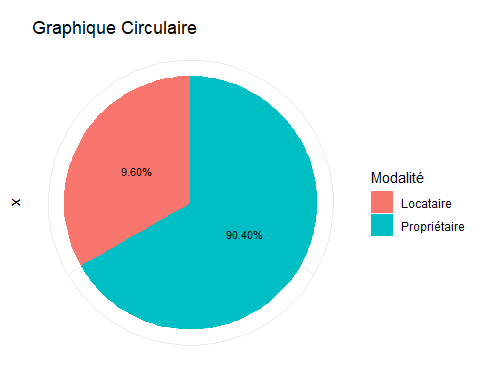
\includegraphics{AWOUTO_Projet_files/figure-latex/unnamed-chunk-17-1.pdf}

Comme on pouvait l'attendre les PME( soit 90\%) possèdent les surfaces
cultivées où ils travaiillent.

\hypertarget{repartition-des-pme-selon-le-statut-juridique-le-statut-juridique-et-le-sexe}{%
\subparagraph{2.1.4.5 Repartition des PME selon le Statut juridique le
statut juridique et le
sexe}\label{repartition-des-pme-selon-le-statut-juridique-le-statut-juridique-et-le-sexe}}

\begin{Shaded}
\begin{Highlighting}[]
\FunctionTok{tableau\_croise}\NormalTok{(projet}\SpecialCharTok{$}\StringTok{\textasciigrave{}}\AttributeTok{Statut juridique}\StringTok{\textasciigrave{}}\NormalTok{, projet}\SpecialCharTok{$}\NormalTok{sexe)}
\end{Highlighting}
\end{Shaded}

\begin{verbatim}
##              var2
## var1          Femme Homme Total
##   Association     3     3     6
##   GIE           149    30   179
##   Informel       32     6    38
##   SA              1     6     7
##   SARL            2    11    13
##   SUARL           4     3     7
##   Total         191    59   250
\end{verbatim}

\hypertarget{repartition-des-pme-selon-la-variable-propriuxe9tairelocataire-suivant-le-sexe}{%
\subparagraph{2.1.4.6 Repartition des PME selon la variable
Propriétaire/locataire suivant le
sexe}\label{repartition-des-pme-selon-la-variable-propriuxe9tairelocataire-suivant-le-sexe}}

\begin{Shaded}
\begin{Highlighting}[]
\FunctionTok{tableau\_croise}\NormalTok{(projet}\SpecialCharTok{$}\StringTok{\textasciigrave{}}\AttributeTok{propriétaire ou locataire}\StringTok{\textasciigrave{}}\NormalTok{, projet}\SpecialCharTok{$}\NormalTok{sexe)}
\end{Highlighting}
\end{Shaded}

\begin{verbatim}
##               var2
## var1           Femme Homme Total
##   Locataire       16     8    24
##   Propriétaire   175    51   226
##   Total          191    59   250
\end{verbatim}

\hypertarget{repartition-des-pme-selon-le-statut-juridique-et-le-sexe}{%
\subparagraph{2.1.4.8 Repartition des PME selon le Statut juridique et
le
sexe}\label{repartition-des-pme-selon-le-statut-juridique-et-le-sexe}}

\begin{Shaded}
\begin{Highlighting}[]
\FunctionTok{tableau\_croise}\NormalTok{(projet}\SpecialCharTok{$}\StringTok{\textasciigrave{}}\AttributeTok{Statut juridique}\StringTok{\textasciigrave{}}\NormalTok{, projet}\SpecialCharTok{$}\NormalTok{sexe)}
\end{Highlighting}
\end{Shaded}

\begin{verbatim}
##              var2
## var1          Femme Homme Total
##   Association     3     3     6
##   GIE           149    30   179
##   Informel       32     6    38
##   SA              1     6     7
##   SARL            2    11    13
##   SUARL           4     3     7
##   Total         191    59   250
\end{verbatim}

\hypertarget{statistiques-descriptives-sur-les-autres-variables}{%
\subsection{2.2. Statistiques descriptives sur les autres
variables}\label{statistiques-descriptives-sur-les-autres-variables}}

\hypertarget{cruxe9ation-dune-variable-nommuxe9e-filiere-celle-ci-donne-la-culture-principale-des-pme}{%
\subsubsection{2.2.1 Création d'une variable nommée filiere: Celle ci
donne la culture principale des
PME}\label{cruxe9ation-dune-variable-nommuxe9e-filiere-celle-ci-donne-la-culture-principale-des-pme}}

\begin{Shaded}
\begin{Highlighting}[]
\NormalTok{projet }\OtherTok{\textless{}{-}}\NormalTok{ Projet }\SpecialCharTok{\%\textgreater{}\%} \FunctionTok{mutate}\NormalTok{(}\AttributeTok{filiere =} \FunctionTok{if\_else}\NormalTok{(filiere\_1 }\SpecialCharTok{==}\DecValTok{1}\NormalTok{, }
                  \StringTok{"Arachide"}\NormalTok{,}\FunctionTok{if\_else}\NormalTok{(filiere\_2 }\SpecialCharTok{==}\DecValTok{1}\NormalTok{, }
                  \StringTok{"Anarchade"}\NormalTok{,}\FunctionTok{if\_else}\NormalTok{(filiere\_3 }\SpecialCharTok{==}\DecValTok{1}\NormalTok{, }
                  \StringTok{"Mangue"}\NormalTok{,}\FunctionTok{if\_else}\NormalTok{(filiere\_4 }\SpecialCharTok{==}\DecValTok{1}\NormalTok{,}\StringTok{"Riz"}\NormalTok{,}\StringTok{""}\NormalTok{)))))}
\CommentTok{\# On crée là le nombre de filière pour chaque PME en faisant la somme des }
\CommentTok{\#           variables filières}
\NormalTok{projet }\OtherTok{\textless{}{-}}\NormalTok{ projet }\SpecialCharTok{\%\textgreater{}\%} \FunctionTok{mutate}\NormalTok{(}\AttributeTok{nb\_filiere =}\NormalTok{ filiere\_1 }\SpecialCharTok{+}\NormalTok{ filiere\_2 }\SpecialCharTok{+}\NormalTok{ filiere\_3 }\SpecialCharTok{+}\NormalTok{ filiere\_4)}

\CommentTok{\# On affiche la répartiton des PME par nbre de filière avec gtsummary}
\NormalTok{tableau\_1 }\OtherTok{\textless{}{-}}\NormalTok{ projet[}\StringTok{"nb\_filiere"}\NormalTok{]}\SpecialCharTok{\%\textgreater{}\%}
  \FunctionTok{tbl\_summary}\NormalTok{(}\AttributeTok{label =}\NormalTok{ nb\_filiere }\SpecialCharTok{\textasciitilde{}} \StringTok{"Nombre de filière"}\NormalTok{,}
\NormalTok{  )}
\NormalTok{tableau\_1}
\end{Highlighting}
\end{Shaded}

\begin{longtable}[]{@{}lc@{}}
\toprule\noalign{}
\textbf{Characteristic} & \textbf{N = 250} \\
\midrule\noalign{}
\endhead
\bottomrule\noalign{}
\endlastfoot
Nombre de filière & \\
1 & 171 (68\%) \\
2 & 59 (24\%) \\
3 & 19 (7.6\%) \\
4 & 1 (0.4\%) \\
\end{longtable}

\hypertarget{cruxe9ons-une-fonction-pour-les-tableaux-croisuxe9s-par-filiuxe8re-et-sexe}{%
\subsubsection{2.2.2\# Créons une fonction pour les tableaux croisés par
filière et
sexe}\label{cruxe9ons-une-fonction-pour-les-tableaux-croisuxe9s-par-filiuxe8re-et-sexe}}

\# Ici aussi pour faire analyser la variable sexe par filière d'activité
, nous avons procéder à l'élaborationdes tableaux gtsummary avec
strate.Par suite , nous avons décidé de définir une fonction qui
facilitera les sorties des résultats sur chaque filière. L'objectif est
de fusionner en lignes le tableau créer ppur chaque variable par filière
et ensuite merger en colonne pour les filières.

\begin{Shaded}
\begin{Highlighting}[]
\FunctionTok{theme\_gtsummary\_compact}\NormalTok{(}\AttributeTok{set\_theme =} \ConstantTok{TRUE}\NormalTok{, }\AttributeTok{font\_size =} \ConstantTok{NULL}\NormalTok{)}
      \CommentTok{\#Créons une fonction pour les tableaux croisés par filière et sexe}


\NormalTok{tabl\_fil }\OtherTok{=}\ControlFlowTok{function}\NormalTok{(base\_donnee, num\_var\_filiere\_, nom\_filiere,lab\_var,num\_var)\{}

                         \DocumentationTok{\#\#\# TABLEAU CROISE}
  
\NormalTok{  tableau }\OtherTok{\textless{}{-}}\NormalTok{ base\_donnee }\SpecialCharTok{\%\textgreater{}\%}
\NormalTok{  dplyr}\SpecialCharTok{::}\FunctionTok{select}\NormalTok{(sexe, q25, q12, q81, }\FunctionTok{names}\NormalTok{(base\_donnee[num\_var\_filiere\_]) }
\NormalTok{                ) }\SpecialCharTok{\%\textgreater{}\%}
\NormalTok{  gtsummary}\SpecialCharTok{::}\FunctionTok{tbl\_strata}\NormalTok{(}
    \AttributeTok{strata =} \FunctionTok{names}\NormalTok{(base\_donnee[num\_var\_filiere\_]),}
    \AttributeTok{.tbl\_fun =} \SpecialCharTok{\textasciitilde{}}\NormalTok{ .x }\SpecialCharTok{\%\textgreater{}\%}
\NormalTok{      gtsummary}\SpecialCharTok{::}\FunctionTok{tbl\_cross}\NormalTok{(}
        \AttributeTok{row =} \FunctionTok{names}\NormalTok{(base\_donnee[num\_var]),}
        \AttributeTok{col =}\NormalTok{ sexe,}
        \AttributeTok{percent =} \StringTok{"cell"}\NormalTok{,}
        \AttributeTok{margin =} \ConstantTok{NULL}\NormalTok{,}
        \CommentTok{\#statistic = \textasciitilde{} "\{p\}\% (\{n\})",}
        \CommentTok{\#digits = \textasciitilde{} 2,}
        \AttributeTok{label =} \FunctionTok{list}\NormalTok{(}\FunctionTok{names}\NormalTok{(base\_donnee[num\_var]) }\SpecialCharTok{\textasciitilde{}} \FunctionTok{as.character}\NormalTok{(lab\_var),}
\NormalTok{                     sexe }\SpecialCharTok{\textasciitilde{}} \StringTok{"sexe du responsable"}\NormalTok{)}
\NormalTok{        ) }\SpecialCharTok{\%\textgreater{}\%} \FunctionTok{add\_p}\NormalTok{() }\SpecialCharTok{\%\textgreater{}\%}
      \FunctionTok{bold\_labels}\NormalTok{() }\SpecialCharTok{\%\textgreater{}\%}
      \FunctionTok{italicize\_levels}\NormalTok{(),}
    
    \DocumentationTok{\#\# préciser comment combiner les tableaux de chaque groupe. Par défaut, }
    \DocumentationTok{\#\# il combine avec "tbl\_merge"}
    \AttributeTok{.combine\_with =} \StringTok{"tbl\_merge"}\NormalTok{, }
    \AttributeTok{.header =} \StringTok{"\{strata\}"}
\NormalTok{    )}\SpecialCharTok{\%\textgreater{}\%}
    \DocumentationTok{\#\# mise en forme de l\textquotesingle{}entête du tableau}
   \FunctionTok{modify\_header}\NormalTok{(}
      \FunctionTok{list}\NormalTok{(}
        \FunctionTok{all\_stat\_cols}\NormalTok{(}\AttributeTok{stat\_0 =} \ConstantTok{FALSE}\NormalTok{) }\SpecialCharTok{\textasciitilde{}} \StringTok{"**\{level\}** (n=\{n\}, \{style\_percent(p)\}\%)"}
\NormalTok{      )}
\NormalTok{     ) }\SpecialCharTok{\%\textgreater{}\%} 
    \FunctionTok{modify\_column\_hide}\NormalTok{(}\FunctionTok{c}\NormalTok{(stat\_1\_1,stat\_2\_1,p.value\_1))}
  \FunctionTok{return}\NormalTok{(tableau)}
\NormalTok{\}}

\NormalTok{tab\_prop\_1 }\OtherTok{\textless{}{-}} \FunctionTok{tabl\_fil}\NormalTok{(projet,}\DecValTok{23}\NormalTok{,}\StringTok{"Arachide"}\NormalTok{,}\StringTok{"Propriétaire/Locataire"}\NormalTok{,}
                       \FunctionTok{which}\NormalTok{(}\FunctionTok{names}\NormalTok{(projet)}\SpecialCharTok{==}\StringTok{"q81"}\NormalTok{))}
\NormalTok{tab\_niv\_1 }\OtherTok{\textless{}{-}} \FunctionTok{tabl\_fil}\NormalTok{(projet,}\DecValTok{23}\NormalTok{,}\StringTok{"Arachide"}\NormalTok{,}\StringTok{"Niveau d\textquotesingle{}instruction"}\NormalTok{,}
                      \FunctionTok{which}\NormalTok{(}\FunctionTok{names}\NormalTok{(projet)}\SpecialCharTok{==}\StringTok{"q25"}\NormalTok{))}
\NormalTok{tab\_stat\_1 }\OtherTok{\textless{}{-}} \FunctionTok{tabl\_fil}\NormalTok{(projet,}\DecValTok{23}\NormalTok{,}\StringTok{"Arachide"}\NormalTok{,}\StringTok{"Statut juridique"}\NormalTok{,}
                       \FunctionTok{which}\NormalTok{(}\FunctionTok{names}\NormalTok{(projet)}\SpecialCharTok{==}\StringTok{"q81"}\NormalTok{))}

\NormalTok{tab\_fil\_1 }\OtherTok{\textless{}{-}}\NormalTok{ gtsummary}\SpecialCharTok{::}\FunctionTok{tbl\_stack}\NormalTok{(}\FunctionTok{list}\NormalTok{(tab\_prop\_1, tab\_niv\_1,tab\_stat\_1))}


\NormalTok{tab\_prop\_2 }\OtherTok{\textless{}{-}} \FunctionTok{tabl\_fil}\NormalTok{(projet,}\DecValTok{24}\NormalTok{,}\StringTok{"Anarchade"}\NormalTok{,}\StringTok{"Propriétaire/Locataire"}\NormalTok{,}
                       \FunctionTok{which}\NormalTok{(}\FunctionTok{names}\NormalTok{(projet)}\SpecialCharTok{==}\StringTok{"q81"}\NormalTok{))}
\NormalTok{tab\_niv\_2 }\OtherTok{\textless{}{-}} \FunctionTok{tabl\_fil}\NormalTok{(projet,}\DecValTok{24}\NormalTok{,}\StringTok{"Anarchade"}\NormalTok{,}\StringTok{"Niveau d\textquotesingle{}instruction"}\NormalTok{,}
                      \FunctionTok{which}\NormalTok{(}\FunctionTok{names}\NormalTok{(projet)}\SpecialCharTok{==}\StringTok{"q25"}\NormalTok{))}
\NormalTok{tab\_stat\_2 }\OtherTok{\textless{}{-}} \FunctionTok{tabl\_fil}\NormalTok{(projet,}\DecValTok{24}\NormalTok{,}\StringTok{"Anarchade"}\NormalTok{,}\StringTok{"Statut juridique"}\NormalTok{,}
                       \FunctionTok{which}\NormalTok{(}\FunctionTok{names}\NormalTok{(projet)}\SpecialCharTok{==}\StringTok{"q81"}\NormalTok{))}

\NormalTok{tab\_fil\_2 }\OtherTok{\textless{}{-}}\NormalTok{ gtsummary}\SpecialCharTok{::}\FunctionTok{tbl\_stack}\NormalTok{(}\FunctionTok{list}\NormalTok{(tab\_prop\_2, tab\_niv\_2,tab\_stat\_2))}


\NormalTok{tab\_prop\_3 }\OtherTok{\textless{}{-}} \FunctionTok{tabl\_fil}\NormalTok{(projet,}\DecValTok{25}\NormalTok{,}\StringTok{"Arachide"}\NormalTok{,}\StringTok{"Propriétaire/Locataire"}\NormalTok{,}
                       \FunctionTok{which}\NormalTok{(}\FunctionTok{names}\NormalTok{(projet)}\SpecialCharTok{==}\StringTok{"q81"}\NormalTok{))}
\NormalTok{tab\_niv\_3 }\OtherTok{\textless{}{-}} \FunctionTok{tabl\_fil}\NormalTok{(projet,}\DecValTok{25}\NormalTok{,}\StringTok{"Arachide"}\NormalTok{,}\StringTok{"Niveau d\textquotesingle{}instruction"}\NormalTok{,}
                      \FunctionTok{which}\NormalTok{(}\FunctionTok{names}\NormalTok{(projet)}\SpecialCharTok{==}\StringTok{"q25"}\NormalTok{))}
\NormalTok{tab\_stat\_3 }\OtherTok{\textless{}{-}} \FunctionTok{tabl\_fil}\NormalTok{(projet,}\DecValTok{25}\NormalTok{,}\StringTok{"Arachide"}\NormalTok{,}\StringTok{"Statut juridique"}\NormalTok{,}
                       \FunctionTok{which}\NormalTok{(}\FunctionTok{names}\NormalTok{(projet)}\SpecialCharTok{==}\StringTok{"q81"}\NormalTok{))}

\NormalTok{tab\_fil\_3 }\OtherTok{\textless{}{-}}\NormalTok{ gtsummary}\SpecialCharTok{::}\FunctionTok{tbl\_stack}\NormalTok{(}\FunctionTok{list}\NormalTok{(tab\_prop\_3, tab\_niv\_3,tab\_stat\_3))}

\NormalTok{tab\_prop\_4 }\OtherTok{\textless{}{-}} \FunctionTok{tabl\_fil}\NormalTok{(projet,}\DecValTok{26}\NormalTok{,}\StringTok{"Arachide"}\NormalTok{,}\StringTok{"Propriétaire/Locataire"}\NormalTok{,}
                       \FunctionTok{which}\NormalTok{(}\FunctionTok{names}\NormalTok{(projet)}\SpecialCharTok{==}\StringTok{"q81"}\NormalTok{))}
\NormalTok{tab\_niv\_4 }\OtherTok{\textless{}{-}} \FunctionTok{tabl\_fil}\NormalTok{(projet,}\DecValTok{26}\NormalTok{,}\StringTok{"Arachide"}\NormalTok{,}\StringTok{"Niveau d\textquotesingle{}instruction"}\NormalTok{,}
                      \FunctionTok{which}\NormalTok{(}\FunctionTok{names}\NormalTok{(projet)}\SpecialCharTok{==}\StringTok{"q25"}\NormalTok{))}
\NormalTok{tab\_stat\_4 }\OtherTok{\textless{}{-}} \FunctionTok{tabl\_fil}\NormalTok{(projet,}\DecValTok{26}\NormalTok{,}\StringTok{"Arachide"}\NormalTok{,}\StringTok{"Statut juridique"}\NormalTok{,}
                       \FunctionTok{which}\NormalTok{(}\FunctionTok{names}\NormalTok{(projet)}\SpecialCharTok{==}\StringTok{"q81"}\NormalTok{))}

\NormalTok{tab\_fil\_4 }\OtherTok{\textless{}{-}}\NormalTok{ gtsummary}\SpecialCharTok{::}\FunctionTok{tbl\_stack}\NormalTok{(}\FunctionTok{list}\NormalTok{(tab\_prop\_4, tab\_niv\_4,tab\_stat\_4))}

\NormalTok{tab\_crois }\OtherTok{\textless{}{-}}\NormalTok{ gtsummary}\SpecialCharTok{::}\FunctionTok{tbl\_merge}\NormalTok{(}
  \FunctionTok{list}\NormalTok{(tab\_fil\_1,tab\_fil\_2,tab\_fil\_3,tab\_fil\_4),}
  \AttributeTok{tab\_spanner =} \FunctionTok{c}\NormalTok{(}\StringTok{"**Arachide**"}\NormalTok{, }\StringTok{"**Anacarde**"}\NormalTok{,}\StringTok{"**Mangue**"}\NormalTok{,}\StringTok{"**Riz**"}\NormalTok{) }
  \DocumentationTok{\#\# intitulé des groupes de tableau associés}
\NormalTok{)}
\NormalTok{tab\_crois}
\end{Highlighting}
\end{Shaded}

\begin{longtable}[]{@{}
  >{\raggedright\arraybackslash}p{(\columnwidth - 24\tabcolsep) * \real{0.1027}}
  >{\centering\arraybackslash}p{(\columnwidth - 24\tabcolsep) * \real{0.0875}}
  >{\centering\arraybackslash}p{(\columnwidth - 24\tabcolsep) * \real{0.0875}}
  >{\centering\arraybackslash}p{(\columnwidth - 24\tabcolsep) * \real{0.0494}}
  >{\centering\arraybackslash}p{(\columnwidth - 24\tabcolsep) * \real{0.0875}}
  >{\centering\arraybackslash}p{(\columnwidth - 24\tabcolsep) * \real{0.0875}}
  >{\centering\arraybackslash}p{(\columnwidth - 24\tabcolsep) * \real{0.0494}}
  >{\centering\arraybackslash}p{(\columnwidth - 24\tabcolsep) * \real{0.0875}}
  >{\centering\arraybackslash}p{(\columnwidth - 24\tabcolsep) * \real{0.0875}}
  >{\centering\arraybackslash}p{(\columnwidth - 24\tabcolsep) * \real{0.0494}}
  >{\centering\arraybackslash}p{(\columnwidth - 24\tabcolsep) * \real{0.0875}}
  >{\centering\arraybackslash}p{(\columnwidth - 24\tabcolsep) * \real{0.0875}}
  >{\centering\arraybackslash}p{(\columnwidth - 24\tabcolsep) * \real{0.0494}}@{}}
\toprule\noalign{}
\begin{minipage}[b]{\linewidth}\raggedright
\end{minipage} & \begin{minipage}[b]{\linewidth}\centering
\textbf{Femme} (n=93, 86\%)
\end{minipage} & \begin{minipage}[b]{\linewidth}\centering
\textbf{Homme} (n=15, 14\%)
\end{minipage} & \begin{minipage}[b]{\linewidth}\centering
\textbf{p-value}
\end{minipage} & \begin{minipage}[b]{\linewidth}\centering
\textbf{Femme} (n=40, 66\%)
\end{minipage} & \begin{minipage}[b]{\linewidth}\centering
\textbf{Homme} (n=21, 34\%)
\end{minipage} & \begin{minipage}[b]{\linewidth}\centering
\textbf{p-value}
\end{minipage} & \begin{minipage}[b]{\linewidth}\centering
\textbf{Femme} (n=68, 76\%)
\end{minipage} & \begin{minipage}[b]{\linewidth}\centering
\textbf{Homme} (n=21, 24\%)
\end{minipage} & \begin{minipage}[b]{\linewidth}\centering
\textbf{p-value}
\end{minipage} & \begin{minipage}[b]{\linewidth}\centering
\textbf{Femme} (n=77, 84\%)
\end{minipage} & \begin{minipage}[b]{\linewidth}\centering
\textbf{Homme} (n=15, 16\%)
\end{minipage} & \begin{minipage}[b]{\linewidth}\centering
\textbf{p-value}
\end{minipage} \\
\midrule\noalign{}
\endhead
\bottomrule\noalign{}
\endlastfoot
\textbf{Propriétaire/Locataire} & & & 0.4 & & & 0.2 & & & 0.7 & & &
\textgreater0.9 \\
\emph{Locataire} & 9 (8.3\%) & 3 (2.8\%) & & 3 (4.9\%) & 4 (6.6\%) & & 8
(9.0\%) & 3 (3.4\%) & & 8 (8.7\%) & 1 (1.1\%) & \\
\emph{Propriétaire} & 84 (78\%) & 12 (11\%) & & 37 (61\%) & 17 (28\%) &
& 60 (67\%) & 18 (20\%) & & 69 (75\%) & 14 (15\%) & \\
\textbf{Niveau d'instruction} & & & 0.3 & & & \textless0.001 & & & 0.004
& & & \textless0.001 \\
\emph{Aucun niveau} & 38 (35\%) & 5 (4.6\%) & & 12 (20\%) & 1 (1.6\%) &
& 22 (25\%) & 4 (4.5\%) & & 10 (11\%) & 1 (1.1\%) & \\
\emph{Niveau primaire} & 20 (19\%) & 3 (2.8\%) & & 15 (25\%) & 2 (3.3\%)
& & 20 (22\%) & 4 (4.5\%) & & 26 (28\%) & 0 (0\%) & \\
\emph{Niveau secondaire} & 30 (28\%) & 4 (3.7\%) & & 9 (15\%) & 6
(9.8\%) & & 21 (24\%) & 4 (4.5\%) & & 28 (30\%) & 4 (4.3\%) & \\
\emph{Niveau Superieur} & 5 (4.6\%) & 3 (2.8\%) & & 4 (6.6\%) & 12
(20\%) & & 5 (5.6\%) & 9 (10\%) & & 13 (14\%) & 10 (11\%) & \\
\textbf{Statut juridique} & & & 0.4 & & & 0.2 & & & 0.7 & & &
\textgreater0.9 \\
\emph{Locataire} & 9 (8.3\%) & 3 (2.8\%) & & 3 (4.9\%) & 4 (6.6\%) & & 8
(9.0\%) & 3 (3.4\%) & & 8 (8.7\%) & 1 (1.1\%) & \\
\emph{Propriétaire} & 84 (78\%) & 12 (11\%) & & 37 (61\%) & 17 (28\%) &
& 60 (67\%) & 18 (20\%) & & 69 (75\%) & 14 (15\%) & \\
\end{longtable}

\hypertarget{type-de-filiuxe8re-par-ruxe9gion}{%
\paragraph{2.2.3 Type de filière par
région}\label{type-de-filiuxe8re-par-ruxe9gion}}

Pour une vue assez bonne de la répartition on se limiter à l'analyse de
la vriable region suivant les différentes filières. C'est de ça dont il
est question dans ce code :

\begin{Shaded}
\begin{Highlighting}[]
\FunctionTok{theme\_gtsummary\_compact}\NormalTok{(}\AttributeTok{set\_theme =} \ConstantTok{TRUE}\NormalTok{, }\AttributeTok{font\_size =} \ConstantTok{NULL}\NormalTok{)}

\DocumentationTok{\#\# Format de la sortie}
\FunctionTok{theme\_gtsummary\_printer}\NormalTok{(}
  \AttributeTok{print\_engine =} \StringTok{"flextable"}\NormalTok{,  }
  \CommentTok{\#c("gt", "kable", "kable\_extra", "flextable", "huxtable", "tibble"),}
  \AttributeTok{set\_theme =} \ConstantTok{TRUE}
\NormalTok{)}
               \CommentTok{\# Créons le tableau 1 pour arachide}

\NormalTok{tbl\_1 }\OtherTok{\textless{}{-}}\NormalTok{ projet }\SpecialCharTok{\%\textgreater{}\%}\FunctionTok{select}\NormalTok{(region,filiere\_1) }\SpecialCharTok{\%\textgreater{}\%}
\NormalTok{  gtsummary}\SpecialCharTok{::}\FunctionTok{tbl\_summary}\NormalTok{(}
    \AttributeTok{include =} \FunctionTok{c}\NormalTok{(region,filiere\_1),}
    \AttributeTok{by =}\NormalTok{ filiere\_1}
\NormalTok{  ,}\AttributeTok{label =} \FunctionTok{list}\NormalTok{(region }\SpecialCharTok{\textasciitilde{}} \StringTok{"Région"}\NormalTok{))}\SpecialCharTok{\%\textgreater{}\%}
  \FunctionTok{add\_overall}\NormalTok{()}\SpecialCharTok{\%\textgreater{}\%}
  \FunctionTok{bold\_labels}\NormalTok{() }\SpecialCharTok{\%\textgreater{}\%}
  \FunctionTok{italicize\_levels}\NormalTok{()}\SpecialCharTok{\%\textgreater{}\%}\FunctionTok{modify\_column\_hide}\NormalTok{(}\FunctionTok{c}\NormalTok{(stat\_0,stat\_1))}

               \CommentTok{\# Créons le tableau 2 pour anacharde}

\NormalTok{tbl\_2 }\OtherTok{\textless{}{-}}\NormalTok{ projet }\SpecialCharTok{\%\textgreater{}\%}\FunctionTok{select}\NormalTok{(region,filiere\_2) }\SpecialCharTok{\%\textgreater{}\%}
\NormalTok{  gtsummary}\SpecialCharTok{::}\FunctionTok{tbl\_summary}\NormalTok{(}
    \AttributeTok{include =} \FunctionTok{c}\NormalTok{(region,filiere\_2),}
    \AttributeTok{by =}\NormalTok{ filiere\_2}
\NormalTok{  ,}\AttributeTok{label =} \FunctionTok{list}\NormalTok{(region }\SpecialCharTok{\textasciitilde{}} \StringTok{"Région"}\NormalTok{))}\SpecialCharTok{\%\textgreater{}\%}
  \FunctionTok{add\_overall}\NormalTok{()}\SpecialCharTok{\%\textgreater{}\%}
  \FunctionTok{bold\_labels}\NormalTok{() }\SpecialCharTok{\%\textgreater{}\%}
  \FunctionTok{italicize\_levels}\NormalTok{()}\SpecialCharTok{\%\textgreater{}\%}\FunctionTok{modify\_column\_hide}\NormalTok{(}\FunctionTok{c}\NormalTok{(stat\_0,stat\_1))}

               \CommentTok{\# Créons le tableau 3 pour mangue}
\NormalTok{tbl\_3 }\OtherTok{\textless{}{-}}\NormalTok{ projet }\SpecialCharTok{\%\textgreater{}\%}\FunctionTok{select}\NormalTok{(region,filiere\_3) }\SpecialCharTok{\%\textgreater{}\%}
\NormalTok{  gtsummary}\SpecialCharTok{::}\FunctionTok{tbl\_summary}\NormalTok{(}
    \AttributeTok{include =} \FunctionTok{c}\NormalTok{(region,filiere\_3),}
    \AttributeTok{by =}\NormalTok{ filiere\_3}
\NormalTok{  ,}\AttributeTok{label =} \FunctionTok{list}\NormalTok{(region }\SpecialCharTok{\textasciitilde{}} \StringTok{"Région"}\NormalTok{))}\SpecialCharTok{\%\textgreater{}\%}
  \FunctionTok{add\_overall}\NormalTok{()}\SpecialCharTok{\%\textgreater{}\%}
  \FunctionTok{bold\_labels}\NormalTok{() }\SpecialCharTok{\%\textgreater{}\%}
  \FunctionTok{italicize\_levels}\NormalTok{()}\SpecialCharTok{\%\textgreater{}\%}\FunctionTok{modify\_column\_hide}\NormalTok{(}\FunctionTok{c}\NormalTok{(stat\_0,stat\_1))}

               \CommentTok{\# Créons le tableau 4 pour riz}

\NormalTok{tbl\_4 }\OtherTok{\textless{}{-}}\NormalTok{ projet }\SpecialCharTok{\%\textgreater{}\%}\FunctionTok{select}\NormalTok{(region,filiere\_4) }\SpecialCharTok{\%\textgreater{}\%}
\NormalTok{  gtsummary}\SpecialCharTok{::}\FunctionTok{tbl\_summary}\NormalTok{(}
    \AttributeTok{include =} \FunctionTok{c}\NormalTok{(region,filiere\_4),}
    \AttributeTok{by =}\NormalTok{ filiere\_4}
\NormalTok{  ,}\AttributeTok{label =} \FunctionTok{list}\NormalTok{(region }\SpecialCharTok{\textasciitilde{}} \StringTok{"Région"}\NormalTok{))}\SpecialCharTok{\%\textgreater{}\%}
  \FunctionTok{add\_overall}\NormalTok{()}\SpecialCharTok{\%\textgreater{}\%}
  \FunctionTok{bold\_labels}\NormalTok{() }\SpecialCharTok{\%\textgreater{}\%}
  \FunctionTok{italicize\_levels}\NormalTok{()}\SpecialCharTok{\%\textgreater{}\%}\FunctionTok{modify\_column\_hide}\NormalTok{(}\FunctionTok{c}\NormalTok{(stat\_0,stat\_1))}

               \CommentTok{\#F les 4 tableaux ci{-}dessus en un seul tableau}

\NormalTok{gtsummary}\SpecialCharTok{::}\FunctionTok{tbl\_merge}\NormalTok{(}
  \FunctionTok{list}\NormalTok{(tbl\_1,tbl\_2,tbl\_3,tbl\_4),}
  \AttributeTok{tab\_spanner =}  \FunctionTok{c}\NormalTok{(}\StringTok{"Arachide"}\NormalTok{, }\StringTok{"Anacarde"}\NormalTok{,}\StringTok{"Mangue"}\NormalTok{,}\StringTok{"Riz"}\NormalTok{) }
  \DocumentationTok{\#\# intitulé des groupes de tableau associés}
\NormalTok{)}
\end{Highlighting}
\end{Shaded}

\global\setlength{\Oldarrayrulewidth}{\arrayrulewidth}

\global\setlength{\Oldtabcolsep}{\tabcolsep}

\setlength{\tabcolsep}{2pt}

\renewcommand*{\arraystretch}{1.5}



\providecommand{\ascline}[3]{\noalign{\global\arrayrulewidth #1}\arrayrulecolor[HTML]{#2}\cline{#3}}

\begin{longtable}[c]{ccccc}



\ascline{1pt}{000000}{1-5}

\multicolumn{1}{>{}l}{\textcolor[HTML]{000000}{\fontsize{8}{8}\selectfont{\ }}} & \multicolumn{1}{>{}c}{\textcolor[HTML]{000000}{\fontsize{8}{8}\selectfont{Arachide}}} & \multicolumn{1}{>{}c}{\textcolor[HTML]{000000}{\fontsize{8}{8}\selectfont{Anacarde}}} & \multicolumn{1}{>{}c}{\textcolor[HTML]{000000}{\fontsize{8}{8}\selectfont{Mangue}}} & \multicolumn{1}{>{}c}{\textcolor[HTML]{000000}{\fontsize{8}{8}\selectfont{Riz}}} \\

\ascline{1pt}{000000}{1-5}



\multicolumn{1}{>{}l}{\textcolor[HTML]{000000}{\fontsize{8}{8}\selectfont{\textbf{Characteristic}}}} & \multicolumn{1}{>{}c}{\textcolor[HTML]{000000}{\fontsize{8}{8}\selectfont{\textbf{1}}}\textcolor[HTML]{000000}{\fontsize{8}{8}\selectfont{,\ N\ =\ 108}}\textcolor[HTML]{000000}{\fontsize{8}{8}\selectfont{\textsuperscript{1}}}} & \multicolumn{1}{>{}c}{\textcolor[HTML]{000000}{\fontsize{8}{8}\selectfont{\textbf{1}}}\textcolor[HTML]{000000}{\fontsize{8}{8}\selectfont{,\ N\ =\ 61}}\textcolor[HTML]{000000}{\fontsize{8}{8}\selectfont{\textsuperscript{1}}}} & \multicolumn{1}{>{}c}{\textcolor[HTML]{000000}{\fontsize{8}{8}\selectfont{\textbf{1}}}\textcolor[HTML]{000000}{\fontsize{8}{8}\selectfont{,\ N\ =\ 89}}\textcolor[HTML]{000000}{\fontsize{8}{8}\selectfont{\textsuperscript{1}}}} & \multicolumn{1}{>{}c}{\textcolor[HTML]{000000}{\fontsize{8}{8}\selectfont{\textbf{1}}}\textcolor[HTML]{000000}{\fontsize{8}{8}\selectfont{,\ N\ =\ 92}}\textcolor[HTML]{000000}{\fontsize{8}{8}\selectfont{\textsuperscript{1}}}} \\

\ascline{1pt}{000000}{1-5}\endfirsthead 

\ascline{1pt}{000000}{1-5}

\multicolumn{1}{>{}l}{\textcolor[HTML]{000000}{\fontsize{8}{8}\selectfont{\ }}} & \multicolumn{1}{>{}c}{\textcolor[HTML]{000000}{\fontsize{8}{8}\selectfont{Arachide}}} & \multicolumn{1}{>{}c}{\textcolor[HTML]{000000}{\fontsize{8}{8}\selectfont{Anacarde}}} & \multicolumn{1}{>{}c}{\textcolor[HTML]{000000}{\fontsize{8}{8}\selectfont{Mangue}}} & \multicolumn{1}{>{}c}{\textcolor[HTML]{000000}{\fontsize{8}{8}\selectfont{Riz}}} \\

\ascline{1pt}{000000}{1-5}



\multicolumn{1}{>{}l}{\textcolor[HTML]{000000}{\fontsize{8}{8}\selectfont{\textbf{Characteristic}}}} & \multicolumn{1}{>{}c}{\textcolor[HTML]{000000}{\fontsize{8}{8}\selectfont{\textbf{1}}}\textcolor[HTML]{000000}{\fontsize{8}{8}\selectfont{,\ N\ =\ 108}}\textcolor[HTML]{000000}{\fontsize{8}{8}\selectfont{\textsuperscript{1}}}} & \multicolumn{1}{>{}c}{\textcolor[HTML]{000000}{\fontsize{8}{8}\selectfont{\textbf{1}}}\textcolor[HTML]{000000}{\fontsize{8}{8}\selectfont{,\ N\ =\ 61}}\textcolor[HTML]{000000}{\fontsize{8}{8}\selectfont{\textsuperscript{1}}}} & \multicolumn{1}{>{}c}{\textcolor[HTML]{000000}{\fontsize{8}{8}\selectfont{\textbf{1}}}\textcolor[HTML]{000000}{\fontsize{8}{8}\selectfont{,\ N\ =\ 89}}\textcolor[HTML]{000000}{\fontsize{8}{8}\selectfont{\textsuperscript{1}}}} & \multicolumn{1}{>{}c}{\textcolor[HTML]{000000}{\fontsize{8}{8}\selectfont{\textbf{1}}}\textcolor[HTML]{000000}{\fontsize{8}{8}\selectfont{,\ N\ =\ 92}}\textcolor[HTML]{000000}{\fontsize{8}{8}\selectfont{\textsuperscript{1}}}} \\

\ascline{1pt}{000000}{1-5}\endhead



\multicolumn{5}{>{}l}{\textcolor[HTML]{000000}{\fontsize{8}{8}\selectfont{\textsuperscript{1}}}\textcolor[HTML]{000000}{\fontsize{8}{8}\selectfont{n\ (\%)}}} \\

\endlastfoot



\multicolumn{1}{>{}l}{\textcolor[HTML]{000000}{\fontsize{8}{8}\selectfont{\textbf{Région}}}} & \multicolumn{1}{>{}c}{\textcolor[HTML]{000000}{\fontsize{8}{8}\selectfont{}}} & \multicolumn{1}{>{}c}{\textcolor[HTML]{000000}{\fontsize{8}{8}\selectfont{}}} & \multicolumn{1}{>{}c}{\textcolor[HTML]{000000}{\fontsize{8}{8}\selectfont{}}} & \multicolumn{1}{>{}c}{\textcolor[HTML]{000000}{\fontsize{8}{8}\selectfont{}}} \\





\multicolumn{1}{>{}l}{\textcolor[HTML]{000000}{\fontsize{8}{8}\selectfont{\textit{Dakar}}}} & \multicolumn{1}{>{}c}{\textcolor[HTML]{000000}{\fontsize{8}{8}\selectfont{0\ (0\%)}}} & \multicolumn{1}{>{}c}{\textcolor[HTML]{000000}{\fontsize{8}{8}\selectfont{1\ (1.6\%)}}} & \multicolumn{1}{>{}c}{\textcolor[HTML]{000000}{\fontsize{8}{8}\selectfont{0\ (0\%)}}} & \multicolumn{1}{>{}c}{\textcolor[HTML]{000000}{\fontsize{8}{8}\selectfont{1\ (1.1\%)}}} \\





\multicolumn{1}{>{}l}{\textcolor[HTML]{000000}{\fontsize{8}{8}\selectfont{\textit{Diourbel}}}} & \multicolumn{1}{>{}c}{\textcolor[HTML]{000000}{\fontsize{8}{8}\selectfont{33\ (31\%)}}} & \multicolumn{1}{>{}c}{\textcolor[HTML]{000000}{\fontsize{8}{8}\selectfont{0\ (0\%)}}} & \multicolumn{1}{>{}c}{\textcolor[HTML]{000000}{\fontsize{8}{8}\selectfont{1\ (1.1\%)}}} & \multicolumn{1}{>{}c}{\textcolor[HTML]{000000}{\fontsize{8}{8}\selectfont{0\ (0\%)}}} \\





\multicolumn{1}{>{}l}{\textcolor[HTML]{000000}{\fontsize{8}{8}\selectfont{\textit{Fatick}}}} & \multicolumn{1}{>{}c}{\textcolor[HTML]{000000}{\fontsize{8}{8}\selectfont{12\ (11\%)}}} & \multicolumn{1}{>{}c}{\textcolor[HTML]{000000}{\fontsize{8}{8}\selectfont{21\ (34\%)}}} & \multicolumn{1}{>{}c}{\textcolor[HTML]{000000}{\fontsize{8}{8}\selectfont{3\ (3.4\%)}}} & \multicolumn{1}{>{}c}{\textcolor[HTML]{000000}{\fontsize{8}{8}\selectfont{4\ (4.3\%)}}} \\





\multicolumn{1}{>{}l}{\textcolor[HTML]{000000}{\fontsize{8}{8}\selectfont{\textit{Kaffrine}}}} & \multicolumn{1}{>{}c}{\textcolor[HTML]{000000}{\fontsize{8}{8}\selectfont{8\ (7.4\%)}}} & \multicolumn{1}{>{}c}{\textcolor[HTML]{000000}{\fontsize{8}{8}\selectfont{0\ (0\%)}}} & \multicolumn{1}{>{}c}{\textcolor[HTML]{000000}{\fontsize{8}{8}\selectfont{5\ (5.6\%)}}} & \multicolumn{1}{>{}c}{\textcolor[HTML]{000000}{\fontsize{8}{8}\selectfont{1\ (1.1\%)}}} \\





\multicolumn{1}{>{}l}{\textcolor[HTML]{000000}{\fontsize{8}{8}\selectfont{\textit{Kaolack}}}} & \multicolumn{1}{>{}c}{\textcolor[HTML]{000000}{\fontsize{8}{8}\selectfont{20\ (19\%)}}} & \multicolumn{1}{>{}c}{\textcolor[HTML]{000000}{\fontsize{8}{8}\selectfont{0\ (0\%)}}} & \multicolumn{1}{>{}c}{\textcolor[HTML]{000000}{\fontsize{8}{8}\selectfont{7\ (7.9\%)}}} & \multicolumn{1}{>{}c}{\textcolor[HTML]{000000}{\fontsize{8}{8}\selectfont{4\ (4.3\%)}}} \\





\multicolumn{1}{>{}l}{\textcolor[HTML]{000000}{\fontsize{8}{8}\selectfont{\textit{Kolda}}}} & \multicolumn{1}{>{}c}{\textcolor[HTML]{000000}{\fontsize{8}{8}\selectfont{1\ (0.9\%)}}} & \multicolumn{1}{>{}c}{\textcolor[HTML]{000000}{\fontsize{8}{8}\selectfont{5\ (8.2\%)}}} & \multicolumn{1}{>{}c}{\textcolor[HTML]{000000}{\fontsize{8}{8}\selectfont{0\ (0\%)}}} & \multicolumn{1}{>{}c}{\textcolor[HTML]{000000}{\fontsize{8}{8}\selectfont{4\ (4.3\%)}}} \\





\multicolumn{1}{>{}l}{\textcolor[HTML]{000000}{\fontsize{8}{8}\selectfont{\textit{Saint-Louis}}}} & \multicolumn{1}{>{}c}{\textcolor[HTML]{000000}{\fontsize{8}{8}\selectfont{1\ (0.9\%)}}} & \multicolumn{1}{>{}c}{\textcolor[HTML]{000000}{\fontsize{8}{8}\selectfont{0\ (0\%)}}} & \multicolumn{1}{>{}c}{\textcolor[HTML]{000000}{\fontsize{8}{8}\selectfont{42\ (47\%)}}} & \multicolumn{1}{>{}c}{\textcolor[HTML]{000000}{\fontsize{8}{8}\selectfont{0\ (0\%)}}} \\





\multicolumn{1}{>{}l}{\textcolor[HTML]{000000}{\fontsize{8}{8}\selectfont{\textit{Sédhiou}}}} & \multicolumn{1}{>{}c}{\textcolor[HTML]{000000}{\fontsize{8}{8}\selectfont{0\ (0\%)}}} & \multicolumn{1}{>{}c}{\textcolor[HTML]{000000}{\fontsize{8}{8}\selectfont{3\ (4.9\%)}}} & \multicolumn{1}{>{}c}{\textcolor[HTML]{000000}{\fontsize{8}{8}\selectfont{0\ (0\%)}}} & \multicolumn{1}{>{}c}{\textcolor[HTML]{000000}{\fontsize{8}{8}\selectfont{3\ (3.3\%)}}} \\





\multicolumn{1}{>{}l}{\textcolor[HTML]{000000}{\fontsize{8}{8}\selectfont{\textit{Thiès}}}} & \multicolumn{1}{>{}c}{\textcolor[HTML]{000000}{\fontsize{8}{8}\selectfont{27\ (25\%)}}} & \multicolumn{1}{>{}c}{\textcolor[HTML]{000000}{\fontsize{8}{8}\selectfont{0\ (0\%)}}} & \multicolumn{1}{>{}c}{\textcolor[HTML]{000000}{\fontsize{8}{8}\selectfont{25\ (28\%)}}} & \multicolumn{1}{>{}c}{\textcolor[HTML]{000000}{\fontsize{8}{8}\selectfont{32\ (35\%)}}} \\





\multicolumn{1}{>{}l}{\textcolor[HTML]{000000}{\fontsize{8}{8}\selectfont{\textit{Ziguinchor}}}} & \multicolumn{1}{>{}c}{\textcolor[HTML]{000000}{\fontsize{8}{8}\selectfont{6\ (5.6\%)}}} & \multicolumn{1}{>{}c}{\textcolor[HTML]{000000}{\fontsize{8}{8}\selectfont{31\ (51\%)}}} & \multicolumn{1}{>{}c}{\textcolor[HTML]{000000}{\fontsize{8}{8}\selectfont{6\ (6.7\%)}}} & \multicolumn{1}{>{}c}{\textcolor[HTML]{000000}{\fontsize{8}{8}\selectfont{43\ (47\%)}}} \\

\ascline{1pt}{000000}{1-5}



\end{longtable}



\arrayrulecolor[HTML]{000000}

\global\setlength{\arrayrulewidth}{\Oldarrayrulewidth}

\global\setlength{\tabcolsep}{\Oldtabcolsep}

\renewcommand*{\arraystretch}{1}

\hypertarget{type-de-filiuxe8re-par-statut-juridique}{%
\paragraph{2.2.4 Type de filière par Statut
juridique}\label{type-de-filiuxe8re-par-statut-juridique}}

de façon analogue à l'analyse de la Région, on peut analyser les
filières en se trestreingant au statut juridique des PME dans le but
d'apprécier de façon pré-empirique le profil de statut juridique suivant
chaque filière.

\begin{Shaded}
\begin{Highlighting}[]
\FunctionTok{theme\_gtsummary\_compact}\NormalTok{(}\AttributeTok{set\_theme =} \ConstantTok{TRUE}\NormalTok{, }\AttributeTok{font\_size =} \ConstantTok{NULL}\NormalTok{)}

\DocumentationTok{\#\# Format de la sortie}
\FunctionTok{theme\_gtsummary\_printer}\NormalTok{(}
  \AttributeTok{print\_engine =} \StringTok{"flextable"}\NormalTok{,  }
  \CommentTok{\#c("gt", "kable", "kable\_extra", "flextable", "huxtable", "tibble"),}
  \AttributeTok{set\_theme =} \ConstantTok{TRUE}
\NormalTok{)}
               \CommentTok{\# Créons le tableau 1 pour arachide}

\NormalTok{tbl\_1 }\OtherTok{\textless{}{-}}\NormalTok{ projet }\SpecialCharTok{\%\textgreater{}\%}\FunctionTok{select}\NormalTok{(q81,filiere\_1) }\SpecialCharTok{\%\textgreater{}\%}
\NormalTok{  gtsummary}\SpecialCharTok{::}\FunctionTok{tbl\_summary}\NormalTok{(}
    \AttributeTok{include =} \FunctionTok{c}\NormalTok{(q81,filiere\_1),}
    \AttributeTok{by =}\NormalTok{ filiere\_1}
\NormalTok{  ,}\AttributeTok{label =} \FunctionTok{list}\NormalTok{(q81 }\SpecialCharTok{\textasciitilde{}} \StringTok{"STATUT JURIDIQUE"}\NormalTok{))}\SpecialCharTok{\%\textgreater{}\%}
  \FunctionTok{add\_overall}\NormalTok{()}\SpecialCharTok{\%\textgreater{}\%}
  \FunctionTok{bold\_labels}\NormalTok{() }\SpecialCharTok{\%\textgreater{}\%}
  \FunctionTok{italicize\_levels}\NormalTok{()}\SpecialCharTok{\%\textgreater{}\%}\FunctionTok{modify\_column\_hide}\NormalTok{(}\FunctionTok{c}\NormalTok{(stat\_0,stat\_1))}

               \CommentTok{\# Créons le tableau 2 pour anacharde}

\NormalTok{tbl\_2 }\OtherTok{\textless{}{-}}\NormalTok{ projet }\SpecialCharTok{\%\textgreater{}\%}\FunctionTok{select}\NormalTok{(q81,filiere\_2) }\SpecialCharTok{\%\textgreater{}\%}
\NormalTok{  gtsummary}\SpecialCharTok{::}\FunctionTok{tbl\_summary}\NormalTok{(}
    \AttributeTok{include =} \FunctionTok{c}\NormalTok{(q81,filiere\_2),}
    \AttributeTok{by =}\NormalTok{ filiere\_2}
\NormalTok{  ,}\AttributeTok{label =} \FunctionTok{list}\NormalTok{(q81 }\SpecialCharTok{\textasciitilde{}} \StringTok{"STATUT JURIDIQUE"}\NormalTok{))}\SpecialCharTok{\%\textgreater{}\%}
  \FunctionTok{add\_overall}\NormalTok{()}\SpecialCharTok{\%\textgreater{}\%}
  \FunctionTok{bold\_labels}\NormalTok{() }\SpecialCharTok{\%\textgreater{}\%}
  \FunctionTok{italicize\_levels}\NormalTok{()}\SpecialCharTok{\%\textgreater{}\%}\FunctionTok{modify\_column\_hide}\NormalTok{(}\FunctionTok{c}\NormalTok{(stat\_0,stat\_1))}

               \CommentTok{\# Créons le tableau 3 pour mangue}
\NormalTok{tbl\_3 }\OtherTok{\textless{}{-}}\NormalTok{ projet }\SpecialCharTok{\%\textgreater{}\%}\FunctionTok{select}\NormalTok{(q81,filiere\_3) }\SpecialCharTok{\%\textgreater{}\%}
\NormalTok{  gtsummary}\SpecialCharTok{::}\FunctionTok{tbl\_summary}\NormalTok{(}
    \AttributeTok{include =} \FunctionTok{c}\NormalTok{(q81,filiere\_3),}
    \AttributeTok{by =}\NormalTok{ filiere\_3}
\NormalTok{  ,}\AttributeTok{label =} \FunctionTok{list}\NormalTok{(q81 }\SpecialCharTok{\textasciitilde{}} \StringTok{"STATUT JURIDIQUE"}\NormalTok{))}\SpecialCharTok{\%\textgreater{}\%}
  \FunctionTok{add\_overall}\NormalTok{()}\SpecialCharTok{\%\textgreater{}\%}
  \FunctionTok{bold\_labels}\NormalTok{() }\SpecialCharTok{\%\textgreater{}\%}
  \FunctionTok{italicize\_levels}\NormalTok{()}\SpecialCharTok{\%\textgreater{}\%}\FunctionTok{modify\_column\_hide}\NormalTok{(}\FunctionTok{c}\NormalTok{(stat\_0,stat\_1))}

               \CommentTok{\# Créons le tableau 4 pour riz}

\NormalTok{tbl\_4 }\OtherTok{\textless{}{-}}\NormalTok{ projet }\SpecialCharTok{\%\textgreater{}\%}\FunctionTok{select}\NormalTok{(q81,filiere\_4) }\SpecialCharTok{\%\textgreater{}\%}
\NormalTok{  gtsummary}\SpecialCharTok{::}\FunctionTok{tbl\_summary}\NormalTok{(}
    \AttributeTok{include =} \FunctionTok{c}\NormalTok{(q81,filiere\_4),}
    \AttributeTok{by =}\NormalTok{ filiere\_4}
\NormalTok{  ,}\AttributeTok{label =} \FunctionTok{list}\NormalTok{(q81}\SpecialCharTok{\textasciitilde{}} \StringTok{"STATUT JURIDIQUE"}\NormalTok{))}\SpecialCharTok{\%\textgreater{}\%}
  \FunctionTok{add\_overall}\NormalTok{()}\SpecialCharTok{\%\textgreater{}\%}
  \FunctionTok{bold\_labels}\NormalTok{() }\SpecialCharTok{\%\textgreater{}\%}
  \FunctionTok{italicize\_levels}\NormalTok{()}\SpecialCharTok{\%\textgreater{}\%}\FunctionTok{modify\_column\_hide}\NormalTok{(}\FunctionTok{c}\NormalTok{(stat\_0,stat\_1))}

               \CommentTok{\#Mergeons les 4 tableaux ci{-}dessus en un seul tableau}

\NormalTok{gtsummary}\SpecialCharTok{::}\FunctionTok{tbl\_merge}\NormalTok{(}
  \FunctionTok{list}\NormalTok{(tbl\_1,tbl\_2,tbl\_3,tbl\_4),}
  \AttributeTok{tab\_spanner =}  \FunctionTok{c}\NormalTok{(}\StringTok{"Arachide"}\NormalTok{, }\StringTok{"Anacarde"}\NormalTok{,}\StringTok{"Mangue"}\NormalTok{,}\StringTok{"Riz"}\NormalTok{) }
  \DocumentationTok{\#\# intitulé des groupes de tableau associés}
\NormalTok{)}
\end{Highlighting}
\end{Shaded}

\global\setlength{\Oldarrayrulewidth}{\arrayrulewidth}

\global\setlength{\Oldtabcolsep}{\tabcolsep}

\setlength{\tabcolsep}{2pt}

\renewcommand*{\arraystretch}{1.5}



\providecommand{\ascline}[3]{\noalign{\global\arrayrulewidth #1}\arrayrulecolor[HTML]{#2}\cline{#3}}

\begin{longtable}[c]{ccccc}



\ascline{1pt}{000000}{1-5}

\multicolumn{1}{>{}l}{\textcolor[HTML]{000000}{\fontsize{8}{8}\selectfont{\ }}} & \multicolumn{1}{>{}c}{\textcolor[HTML]{000000}{\fontsize{8}{8}\selectfont{Arachide}}} & \multicolumn{1}{>{}c}{\textcolor[HTML]{000000}{\fontsize{8}{8}\selectfont{Anacarde}}} & \multicolumn{1}{>{}c}{\textcolor[HTML]{000000}{\fontsize{8}{8}\selectfont{Mangue}}} & \multicolumn{1}{>{}c}{\textcolor[HTML]{000000}{\fontsize{8}{8}\selectfont{Riz}}} \\

\ascline{1pt}{000000}{1-5}



\multicolumn{1}{>{}l}{\textcolor[HTML]{000000}{\fontsize{8}{8}\selectfont{\textbf{Characteristic}}}} & \multicolumn{1}{>{}c}{\textcolor[HTML]{000000}{\fontsize{8}{8}\selectfont{\textbf{1}}}\textcolor[HTML]{000000}{\fontsize{8}{8}\selectfont{,\ N\ =\ 108}}\textcolor[HTML]{000000}{\fontsize{8}{8}\selectfont{\textsuperscript{1}}}} & \multicolumn{1}{>{}c}{\textcolor[HTML]{000000}{\fontsize{8}{8}\selectfont{\textbf{1}}}\textcolor[HTML]{000000}{\fontsize{8}{8}\selectfont{,\ N\ =\ 61}}\textcolor[HTML]{000000}{\fontsize{8}{8}\selectfont{\textsuperscript{1}}}} & \multicolumn{1}{>{}c}{\textcolor[HTML]{000000}{\fontsize{8}{8}\selectfont{\textbf{1}}}\textcolor[HTML]{000000}{\fontsize{8}{8}\selectfont{,\ N\ =\ 89}}\textcolor[HTML]{000000}{\fontsize{8}{8}\selectfont{\textsuperscript{1}}}} & \multicolumn{1}{>{}c}{\textcolor[HTML]{000000}{\fontsize{8}{8}\selectfont{\textbf{1}}}\textcolor[HTML]{000000}{\fontsize{8}{8}\selectfont{,\ N\ =\ 92}}\textcolor[HTML]{000000}{\fontsize{8}{8}\selectfont{\textsuperscript{1}}}} \\

\ascline{1pt}{000000}{1-5}\endfirsthead 

\ascline{1pt}{000000}{1-5}

\multicolumn{1}{>{}l}{\textcolor[HTML]{000000}{\fontsize{8}{8}\selectfont{\ }}} & \multicolumn{1}{>{}c}{\textcolor[HTML]{000000}{\fontsize{8}{8}\selectfont{Arachide}}} & \multicolumn{1}{>{}c}{\textcolor[HTML]{000000}{\fontsize{8}{8}\selectfont{Anacarde}}} & \multicolumn{1}{>{}c}{\textcolor[HTML]{000000}{\fontsize{8}{8}\selectfont{Mangue}}} & \multicolumn{1}{>{}c}{\textcolor[HTML]{000000}{\fontsize{8}{8}\selectfont{Riz}}} \\

\ascline{1pt}{000000}{1-5}



\multicolumn{1}{>{}l}{\textcolor[HTML]{000000}{\fontsize{8}{8}\selectfont{\textbf{Characteristic}}}} & \multicolumn{1}{>{}c}{\textcolor[HTML]{000000}{\fontsize{8}{8}\selectfont{\textbf{1}}}\textcolor[HTML]{000000}{\fontsize{8}{8}\selectfont{,\ N\ =\ 108}}\textcolor[HTML]{000000}{\fontsize{8}{8}\selectfont{\textsuperscript{1}}}} & \multicolumn{1}{>{}c}{\textcolor[HTML]{000000}{\fontsize{8}{8}\selectfont{\textbf{1}}}\textcolor[HTML]{000000}{\fontsize{8}{8}\selectfont{,\ N\ =\ 61}}\textcolor[HTML]{000000}{\fontsize{8}{8}\selectfont{\textsuperscript{1}}}} & \multicolumn{1}{>{}c}{\textcolor[HTML]{000000}{\fontsize{8}{8}\selectfont{\textbf{1}}}\textcolor[HTML]{000000}{\fontsize{8}{8}\selectfont{,\ N\ =\ 89}}\textcolor[HTML]{000000}{\fontsize{8}{8}\selectfont{\textsuperscript{1}}}} & \multicolumn{1}{>{}c}{\textcolor[HTML]{000000}{\fontsize{8}{8}\selectfont{\textbf{1}}}\textcolor[HTML]{000000}{\fontsize{8}{8}\selectfont{,\ N\ =\ 92}}\textcolor[HTML]{000000}{\fontsize{8}{8}\selectfont{\textsuperscript{1}}}} \\

\ascline{1pt}{000000}{1-5}\endhead



\multicolumn{5}{>{}l}{\textcolor[HTML]{000000}{\fontsize{8}{8}\selectfont{\textsuperscript{1}}}\textcolor[HTML]{000000}{\fontsize{8}{8}\selectfont{n\ (\%)}}} \\

\endlastfoot



\multicolumn{1}{>{}l}{\textcolor[HTML]{000000}{\fontsize{8}{8}\selectfont{\textbf{STATUT\ JURIDIQUE}}}} & \multicolumn{1}{>{}c}{\textcolor[HTML]{000000}{\fontsize{8}{8}\selectfont{}}} & \multicolumn{1}{>{}c}{\textcolor[HTML]{000000}{\fontsize{8}{8}\selectfont{}}} & \multicolumn{1}{>{}c}{\textcolor[HTML]{000000}{\fontsize{8}{8}\selectfont{}}} & \multicolumn{1}{>{}c}{\textcolor[HTML]{000000}{\fontsize{8}{8}\selectfont{}}} \\





\multicolumn{1}{>{}l}{\textcolor[HTML]{000000}{\fontsize{8}{8}\selectfont{\textit{Locataire}}}} & \multicolumn{1}{>{}c}{\textcolor[HTML]{000000}{\fontsize{8}{8}\selectfont{12\ (11\%)}}} & \multicolumn{1}{>{}c}{\textcolor[HTML]{000000}{\fontsize{8}{8}\selectfont{7\ (11\%)}}} & \multicolumn{1}{>{}c}{\textcolor[HTML]{000000}{\fontsize{8}{8}\selectfont{11\ (12\%)}}} & \multicolumn{1}{>{}c}{\textcolor[HTML]{000000}{\fontsize{8}{8}\selectfont{9\ (9.8\%)}}} \\





\multicolumn{1}{>{}l}{\textcolor[HTML]{000000}{\fontsize{8}{8}\selectfont{\textit{Propriétaire}}}} & \multicolumn{1}{>{}c}{\textcolor[HTML]{000000}{\fontsize{8}{8}\selectfont{96\ (89\%)}}} & \multicolumn{1}{>{}c}{\textcolor[HTML]{000000}{\fontsize{8}{8}\selectfont{54\ (89\%)}}} & \multicolumn{1}{>{}c}{\textcolor[HTML]{000000}{\fontsize{8}{8}\selectfont{78\ (88\%)}}} & \multicolumn{1}{>{}c}{\textcolor[HTML]{000000}{\fontsize{8}{8}\selectfont{83\ (90\%)}}} \\

\ascline{1pt}{000000}{1-5}



\end{longtable}



\arrayrulecolor[HTML]{000000}

\global\setlength{\arrayrulewidth}{\Oldarrayrulewidth}

\global\setlength{\tabcolsep}{\Oldtabcolsep}

\renewcommand*{\arraystretch}{1}

\hypertarget{manipulation-sur-les-dates-duruxe9e-et-duruxe9e-moyenne-de-lentretien}{%
\subsubsection{2.2.5. Manipulation sur les dates: Durée et Durée moyenne
de
l'entretien}\label{manipulation-sur-les-dates-duruxe9e-et-duruxe9e-moyenne-de-lentretien}}

Cettr sectione est important en ce sens qu'il permet de manipuler le
facteur temps dans notre base de données on peut en effet jouer ou
consulter le temps pour apprécier certaines singularités dans une base
de données.

On peut alors commencer comme suite:

\begin{Shaded}
\begin{Highlighting}[]
\CommentTok{\#Calculer la durée de l’entretien et indiquer la durée moyenne de l’entretien }
\CommentTok{\#                     par enquêteur.}

          \CommentTok{\#Créons d\textquotesingle{}abord la colonne durée de l\textquotesingle{}entretien}

\NormalTok{projet }\OtherTok{\textless{}{-}}\NormalTok{ projet }\SpecialCharTok{\%\textgreater{}\%}
  \FunctionTok{mutate}\NormalTok{(}\AttributeTok{duree\_enquete =} \FunctionTok{interval}\NormalTok{(today,submissiondate) }\SpecialCharTok{\%\textgreater{}\%} \FunctionTok{as.duration}\NormalTok{())}

\CommentTok{\#     Moyenne du temps d\textquotesingle{}un entretien}

\NormalTok{vue\_date }\OtherTok{\textless{}{-}}\NormalTok{projet }\SpecialCharTok{\%\textgreater{}\%} \FunctionTok{group\_by}\NormalTok{(duree\_enquete) }\SpecialCharTok{\%\textgreater{}\%} \FunctionTok{summarise}\NormalTok{(}
  \AttributeTok{Duree\_Moyenne =} \FunctionTok{mean}\NormalTok{(duree\_enquete))}
\FunctionTok{print}\NormalTok{(}\FunctionTok{head}\NormalTok{(vue\_date))}
\end{Highlighting}
\end{Shaded}

\begin{verbatim}
## # A tibble: 6 x 2
##   duree_enquete         Duree_Moyenne
##   <Duration>                    <dbl>
## 1 47463s (~13.18 hours)         47463
## 2 49318s (~13.7 hours)          49318
## 3 49915s (~13.87 hours)         49915
## 4 52658s (~14.63 hours)         52658
## 5 53344s (~14.82 hours)         53344
## 6 55886s (~15.52 hours)         55886
\end{verbatim}

\hypertarget{traitement-sur-les-date}{%
\subsubsection{2.2.6. Traitement sur les
date}\label{traitement-sur-les-date}}

Création des colonnes mois, jour, heure, minutes et temps mis avant de
soumettre en minutes donne un apperçu plus simplifié de l'agrégation du
temps associé à la période d'enquête

\begin{Shaded}
\begin{Highlighting}[]
\NormalTok{projet}\SpecialCharTok{$}\NormalTok{submissiondate }\OtherTok{\textless{}{-}} \FunctionTok{as.POSIXct}\NormalTok{(projet}\SpecialCharTok{$}\NormalTok{submissiondate)}

\CommentTok{\# Ajouter les variables pour le jour, l\textquotesingle{}heure, la minute, le mois de l\textquotesingle{}entretien et la durée de l\textquotesingle{}entretien}
\NormalTok{projet }\OtherTok{\textless{}{-}}\NormalTok{ projet }\SpecialCharTok{\%\textgreater{}\%}
  \FunctionTok{mutate}\NormalTok{( }\AttributeTok{mois\_entretien =} \FunctionTok{format}\NormalTok{(submissiondate, }\StringTok{"\%m"}\NormalTok{),}
         \AttributeTok{jour\_entretien =} \FunctionTok{format}\NormalTok{(submissiondate, }\StringTok{"\%d"}\NormalTok{),}
         \AttributeTok{heure\_entretien =} \FunctionTok{format}\NormalTok{(submissiondate, }\StringTok{"\%H"}\NormalTok{),}
         \AttributeTok{minute\_entretien =} \FunctionTok{format}\NormalTok{(submissiondate, }\StringTok{"\%M"}\NormalTok{),}
         \AttributeTok{duree\_entretien =} \FunctionTok{as.numeric}\NormalTok{(}\FunctionTok{difftime}\NormalTok{(submissiondate, start, }\AttributeTok{units =} \StringTok{"mins"}\NormalTok{)))}
\FunctionTok{print}\NormalTok{(}\FunctionTok{head}\NormalTok{(projet))}
\end{Highlighting}
\end{Shaded}

\begin{verbatim}
## # A tibble: 6 x 41
##   key   region departement sexe    q24 q24a_1 q24a_2 q24a_3 q24a_4 q24a_5 q24a_6
##   <chr> <chr>  <chr>       <chr> <dbl>  <dbl>  <dbl>  <dbl>  <dbl>  <dbl>  <dbl>
## 1 uuid~ Diour~ Bambey      Femme    65      0      1      0      1      0      0
## 2 uuid~ Thiès  Mbour       Femme    52      1      1      0      0      1      0
## 3 uuid~ Thiès  Mbour       Femme    65      1      1      0      0      0      0
## 4 uuid~ Thiès  Mbour       Femme    38      1      1      0      0      1      0
## 5 uuid~ Zigui~ Bignona     Homme    40      1      1      1      0      0      1
## 6 uuid~ Zigui~ Oussouye    Femme    43      1      1      1      0      0      0
## # i 30 more variables: q24a_7 <dbl>, q24a_9 <dbl>, q24a_10 <dbl>, q25 <chr>,
## #   q26 <dbl>, q12 <chr>, q14b <chr>, q16 <chr>, q17 <chr>, q19 <chr>,
## #   q20 <chr>, filiere_1 <dbl>, filiere_2 <dbl>, filiere_3 <dbl>,
## #   filiere_4 <dbl>, q8 <chr>, q81 <chr>, gps_menlatitude <dbl>,
## #   gps_menlongitude <dbl>, submissiondate <dttm>, start <dttm>, today <dttm>,
## #   filiere <chr>, nb_filiere <dbl>, duree_enquete <Duration>,
## #   mois_entretien <chr>, jour_entretien <chr>, heure_entretien <chr>, ...
\end{verbatim}

\hypertarget{cruxe9ation-de-fonction-dextration-conditionnuxe9e-par-une-date}{%
\section{\#\#\# 2.2.7.création de fonction d'extration conditionnée par
une
date}\label{cruxe9ation-de-fonction-dextration-conditionnuxe9e-par-une-date}}

\begin{Shaded}
\begin{Highlighting}[]
\FunctionTok{library}\NormalTok{(dplyr)}

\NormalTok{extraire\_soumissions\_avant\_date }\OtherTok{\textless{}{-}} \ControlFlowTok{function}\NormalTok{(base, date\_limite) \{}
  \CommentTok{\# Convertir la variable submissiondate en un objet de date/heure}
\NormalTok{  base}\SpecialCharTok{$}\NormalTok{submissiondate }\OtherTok{\textless{}{-}} \FunctionTok{as.POSIXct}\NormalTok{(base}\SpecialCharTok{$}\NormalTok{submissiondate)}
  
  \CommentTok{\# Extraire les soumissions avant la date limite}
\NormalTok{  soumissions\_avant\_date }\OtherTok{\textless{}{-}}\NormalTok{ base }\SpecialCharTok{\%\textgreater{}\%}
    \FunctionTok{filter}\NormalTok{(submissiondate }\SpecialCharTok{\textless{}}\NormalTok{ date\_limite)}
  
  \FunctionTok{return}\NormalTok{(soumissions\_avant\_date)}
\NormalTok{\}}
\end{Highlighting}
\end{Shaded}

Exemple d'utilisation de la fonction avec une date donnée (par exemple,
le 05 juin 2023) dont je souligne que ça été pris de façon aléatoire.
Dans une enquête, cette date ou toute autre autre date peut bien jouer
un rôle

\begin{Shaded}
\begin{Highlighting}[]
\NormalTok{date\_limite }\OtherTok{\textless{}{-}} \FunctionTok{as.POSIXct}\NormalTok{(}\StringTok{"2021{-}06{-}05"}\NormalTok{)}
\NormalTok{soumissions\_avant\_date }\OtherTok{\textless{}{-}} \FunctionTok{extraire\_soumissions\_avant\_date}\NormalTok{(projet, date\_limite)}

\CommentTok{\# Vérifier les soumissions extraites}
\FunctionTok{head}\NormalTok{(soumissions\_avant\_date)}
\end{Highlighting}
\end{Shaded}

\begin{verbatim}
## # A tibble: 6 x 41
##   key   region departement sexe    q24 q24a_1 q24a_2 q24a_3 q24a_4 q24a_5 q24a_6
##   <chr> <chr>  <chr>       <chr> <dbl>  <dbl>  <dbl>  <dbl>  <dbl>  <dbl>  <dbl>
## 1 uuid~ Thiès  Mbour       Femme    65      1      1      0      0      0      0
## 2 uuid~ Zigui~ Bignona     Homme    40      1      1      1      0      0      1
## 3 uuid~ Zigui~ Ziguinchor  Homme    33      1      0      0      0      0      0
## 4 uuid~ Thiès  Thiès       Femme    45      0      1      0      0      0      0
## 5 uuid~ Sédhi~ Goudomp     Homme    47      1      0      0      0      0      1
## 6 uuid~ Zigui~ Ziguinchor  Homme    54      0      1      0      0      1      1
## # i 30 more variables: q24a_7 <dbl>, q24a_9 <dbl>, q24a_10 <dbl>, q25 <chr>,
## #   q26 <dbl>, q12 <chr>, q14b <chr>, q16 <chr>, q17 <chr>, q19 <chr>,
## #   q20 <chr>, filiere_1 <dbl>, filiere_2 <dbl>, filiere_3 <dbl>,
## #   filiere_4 <dbl>, q8 <chr>, q81 <chr>, gps_menlatitude <dbl>,
## #   gps_menlongitude <dbl>, submissiondate <dttm>, start <dttm>, today <dttm>,
## #   filiere <chr>, nb_filiere <dbl>, duree_enquete <Duration>,
## #   mois_entretien <chr>, jour_entretien <chr>, heure_entretien <chr>, ...
\end{verbatim}

\end{document}
